	
\part{Cinética de crescimento}
	\chapter{SAXS resolvido no tempo}
	O objetivo desta seção é determinar a cinética de crescimento de micelas de surfactantes catiônicos e NaSal, tanto por SAXS resolvido no tempo quanto por fluorescência resolvida no tempo. Esse estudo foi realizado para verificar se os picos secundários vistos na \autoref{fig:itc_raw_agua_glicerina} são devido ao crescimento micelar, ou a algum outro processo.
	
	\section{Estudos preliminares} 
	Antes de iniciar as medidas de SAXS resolvido no tempo, foram testadas várias amostras para observar qual é a combinação de surfactante e cossoluto com mais contraste, e que possui maior diferença entre os estados iniciais e finais. Foram escolhidos \CTAB, \TTAB{} e \DTAB{} com surfactantes, inicialmente, mas \CTAB{} foi descartado rapidamente pois a temperatura ambiente era menor do que o ponto Krafft do surfactante, e haveria a precipitação do mesmo dentro das seringas de injeção. Como cossoluto, escolheu-se NaSal, 4-clorobenzoato e 3,4-diclorobenzoato. Os cossolutos clorados apresentariam maior contraste, por possuírem maior densidade eletrônica, e por isso foram escolhidos.
	
	Foram preparadas soluções nas concentrações de 100 \mM{} de surfactante, que caracteriza o estado antes do crescimento, e 100 \mM{} de surfactante com 100 \mM{} do cossoluto, que caracteriza o estado depois do crescimento. Após o preparo e estabilização das amostras, as mesmas foram injetadas no capilar de \emph{flow-through} do equipamento. As curvas adquiridas estão na \autoref{fig:ft_preliminar}. Não foi incluída a mistura 3,4-diclorobenzoato e surfactante, pois o contraste era muito baixo, e não havia uma boa relação sinal-ruído.
	
	\begin{figure}[h]
		\centering
		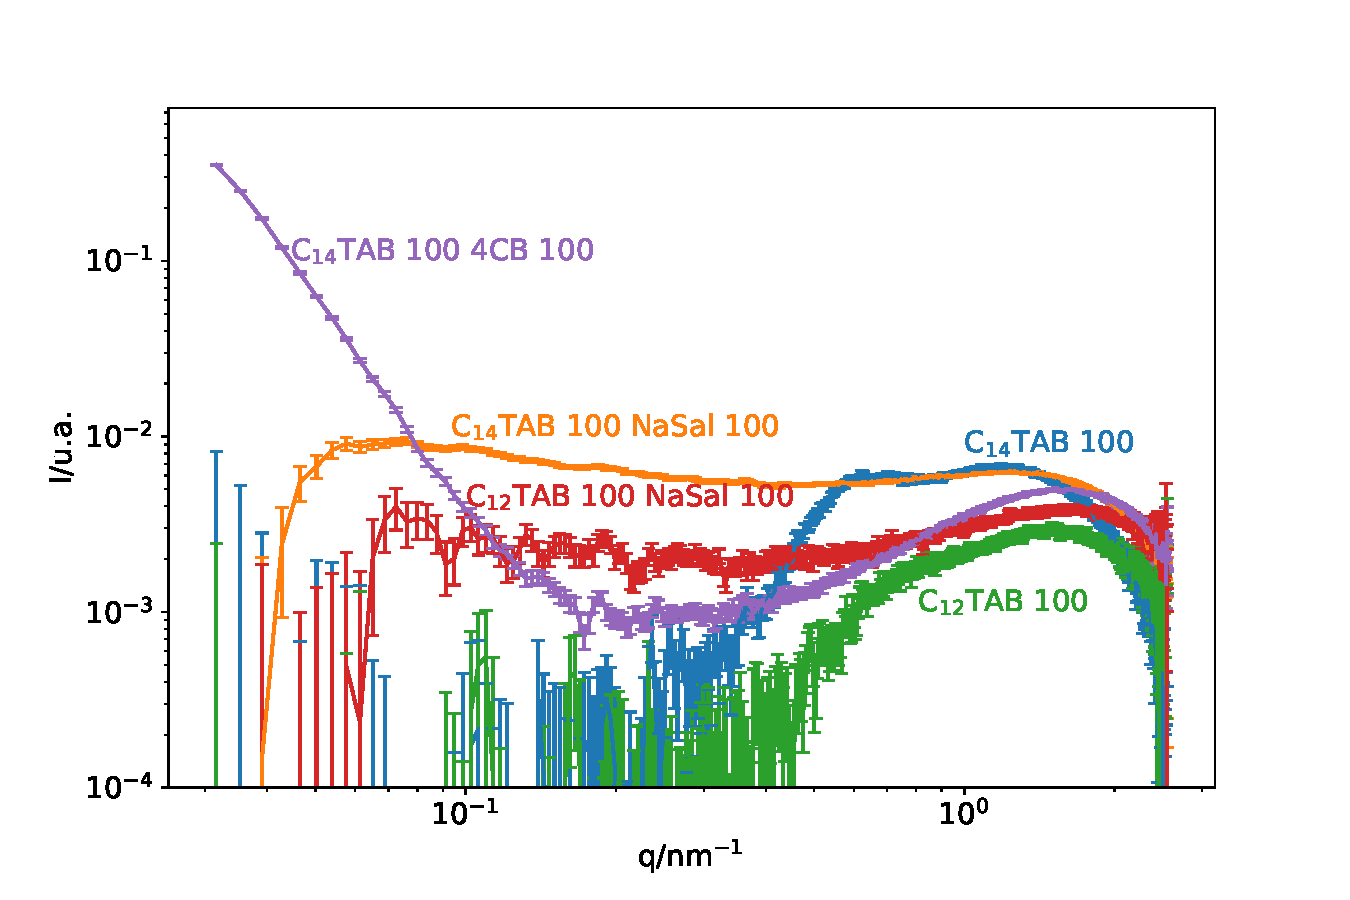
\includegraphics[width=0.7\textwidth]{imagens/saxs/FT_amostras}
		\caption{Curvas de SAXS para várias misturas de surfactantes e cossolutos, com 100 ms de tempo de integração.}
		\label{fig:ft_preliminar}
	\end{figure}

	Observando as curvas, é possível notar que a diferença entre os estados iniciais e finais de \DTAB{} não são muito diferentes, possivelmente porque as micelas formadas não possuem um comprimento muito significativo. Já a diferença entre os estados iniciais e finais para \TTAB{} é bastante pronunciada. Um gráfico comparativo foi criado, realçando as regiões de maior importância (\autoref{fig:tr_comparacao_ttab}).
	
	\begin{figure}[h]
		\centering
		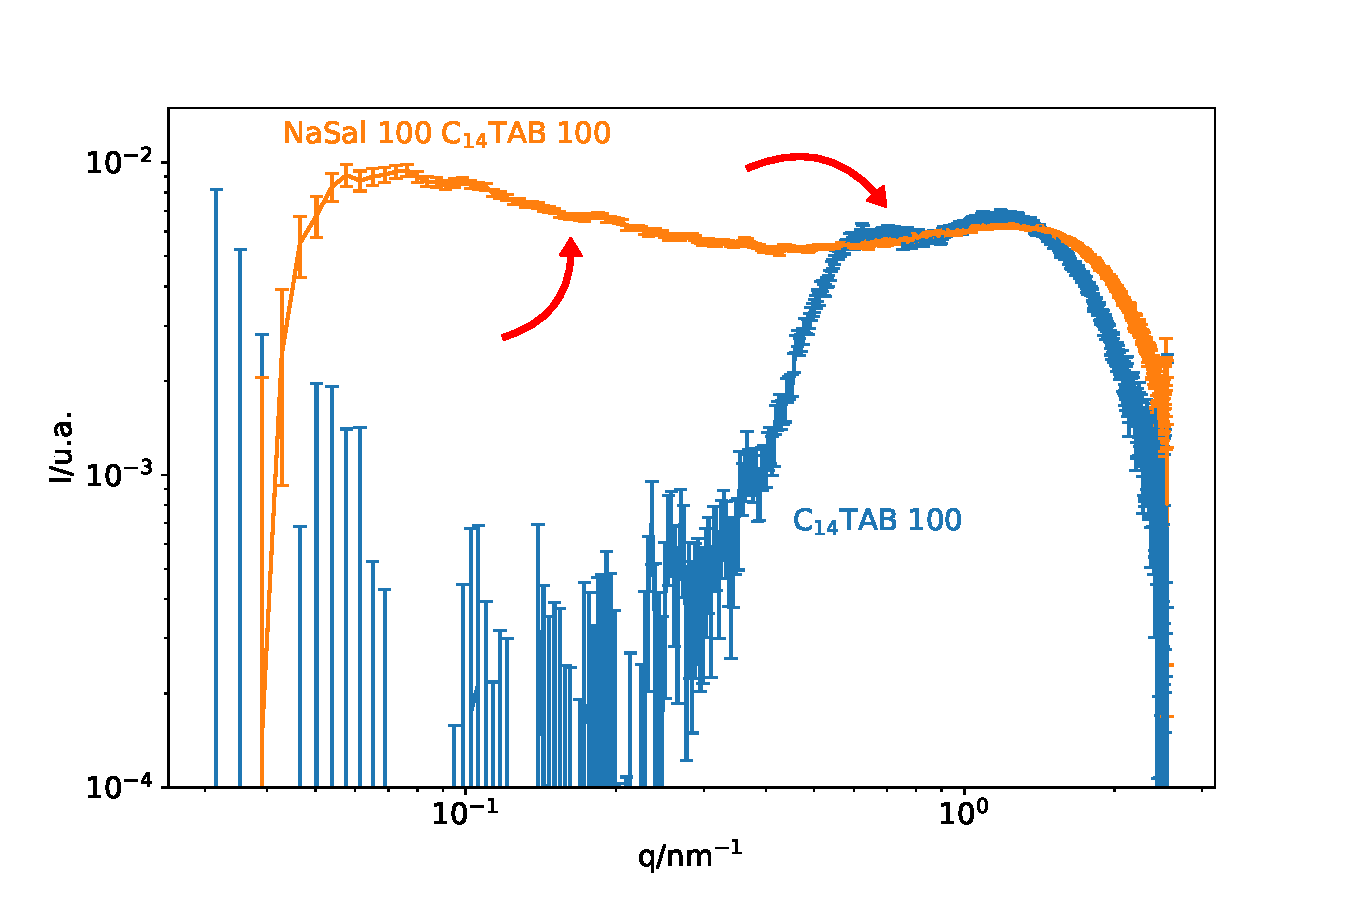
\includegraphics[width=0.7\textwidth]{imagens/saxs/tr_comparacao_antes_depois}
		\caption{Curvas de SAXS para amostras de \TTAB{} 100\mM{} (antes) e 100 \mM de \TTAB{} com 100 \mM{} de NaSal (depois). As setas indicam as regiões onde será observada a maior diferença nas curvas.}
		\label{fig:tr_comparacao_ttab}
	\end{figure}
	
	A região em baixos valores de \q{} é bastante ruidosa na amostra com \TTAB{} 100 \mM{} devido ao baixo contraste entre a amostra e o \emph{background}. O mesmo ocorre na amostra com micelas gigantes de NaSal e \TTAB, e a queda na curva não possui significado físico. Isso será importante na discussão, pois observar-se-á que essa região terá um decaimento em \(q^{-4}\), que pode não ter significado físico, e é um artefato oriundo do baixo contraste. É interessante notar a semelhança entre o perfil de espalhamento obtido aqui e na \autoref{fig:SAXS_micelas_esfericas}, obtido na linha SAXS1 do LNLS. A principal diferença é uma faixa de \q{} menor, que fornece informações sobre estruturas maiores, o que é mais apropriado ao estudo de micelas gigantes.
	
	\section{TR-SAXS} \index{resultados!SAXS!resolvido no tempo}
	\label{sec:tr-saxs}
	Com essas informações, foram medidas várias misturas de \TTAB{} e NaSal, nas proporções de 55:55, 75:75, 100:100 e 60:100 de NaSal:TTAB. Todas as concentrações estão em \mM. Com essas variações de concentração, era esperado observar mudanças na cinética de crescimento. A amostra com 60:100 NaSal:TTAB foi escolhida por possuir uma carga positiva e, consequentemente, resultar numa solução micelar mais viscosa, cujo crescimento poderia ser mais lento também. Essa última amostra foi medida em duas distâncias de detector, 3 m e 1,5 m, para ver se isso afetava os resultados dos ajustes. Todas as outras amostras foram medidas com o detector a 3 m de distância.
	
	Várias combinações de tempos de espera foram estudadas, e no final concluiu-se que os parâmetros disponíveis na \autoref{tab:ccdmvdc_par} forneceram a melhor razão sinal-ruído com o menor tempo possível de integração. Com esses parâmetros pode-se calcular o tempo desde a mistura inicial até um determinado \emph{frame}. Para as amostras analisadas, os tempos do início de cada \emph{frame} estão na \autoref{tab:tr_tempos_frames}.
	
				\begin{table}[h]
		\IBGEtab{%
			\caption{Tempos de mistura no início de cada \emph{frame} para as análises de SAXS resolvido no tempo}
			\label{tab:tr_tempos_frames}
		}%
		{%
			\begin{tabular}{c c | c c | c c | c c | c c}
				\toprule
				Frame & Tempo/s & Frame & Tempo/s & Frame & Tempo/s & Frame & Tempo/s & Frame & Tempo/s \\ \midrule
				  1   & 0.035   & 7     & 0.249   & 13    & 0.583   & 19    & 1.127   & 25    & 2.045   \\
				  2   & 0.065   & 8     & 0.295   & 14    & 0.655   & 20    & 1.248   & 26    & 2.252   \\
				  3   & 0.097   & 9     & 0.344   & 15    & 0.734   & 21    & 1.380   & 27    & 2.479   \\
				  4   & 0.131   & 10    & 0.397   & 16    & 0.820   & 22    & 1.525   & 28    & 2.727   \\
				  5   & 0.168   & 11    & 0.454   & 17    & 0.914   & 23    & 1.683   & 29    & 2.999   \\
				  6   & 0.207   & 12    & 0.516   & 18    & 1.016   & 24    & 1.856   & 30    & 3.298	\\ \bottomrule
			\end{tabular}
		}{}
	\end{table}  
	
	Cada combinação NaSal:TTAB foi analisada no mínimo 5 vezes, e foi feita uma média das curvas, com propagação de erro. Cada curva foi analisada pelo software SUPERSAXS. As Figuras \ref{fig:saxs_tr_55}, \ref{fig:saxs_tr_75}, \ref{fig:saxs_tr_100}, \ref{fig:saxs_tr_60_3} e \ref{fig:saxs_tr_60_15} mostram os dados obtidos e os ajustes de cada uma das curvas médias. As curvas estão coloridas de modo que as primeiras estejam em tons escuros e as últimas, em tons claros. Os números dos \emph{frames} estão juntos de cada cor em cada figura.
	
	\begin{figure}[h]
		\begin{subfigure}[t]{0.5\textwidth}
			\centering
			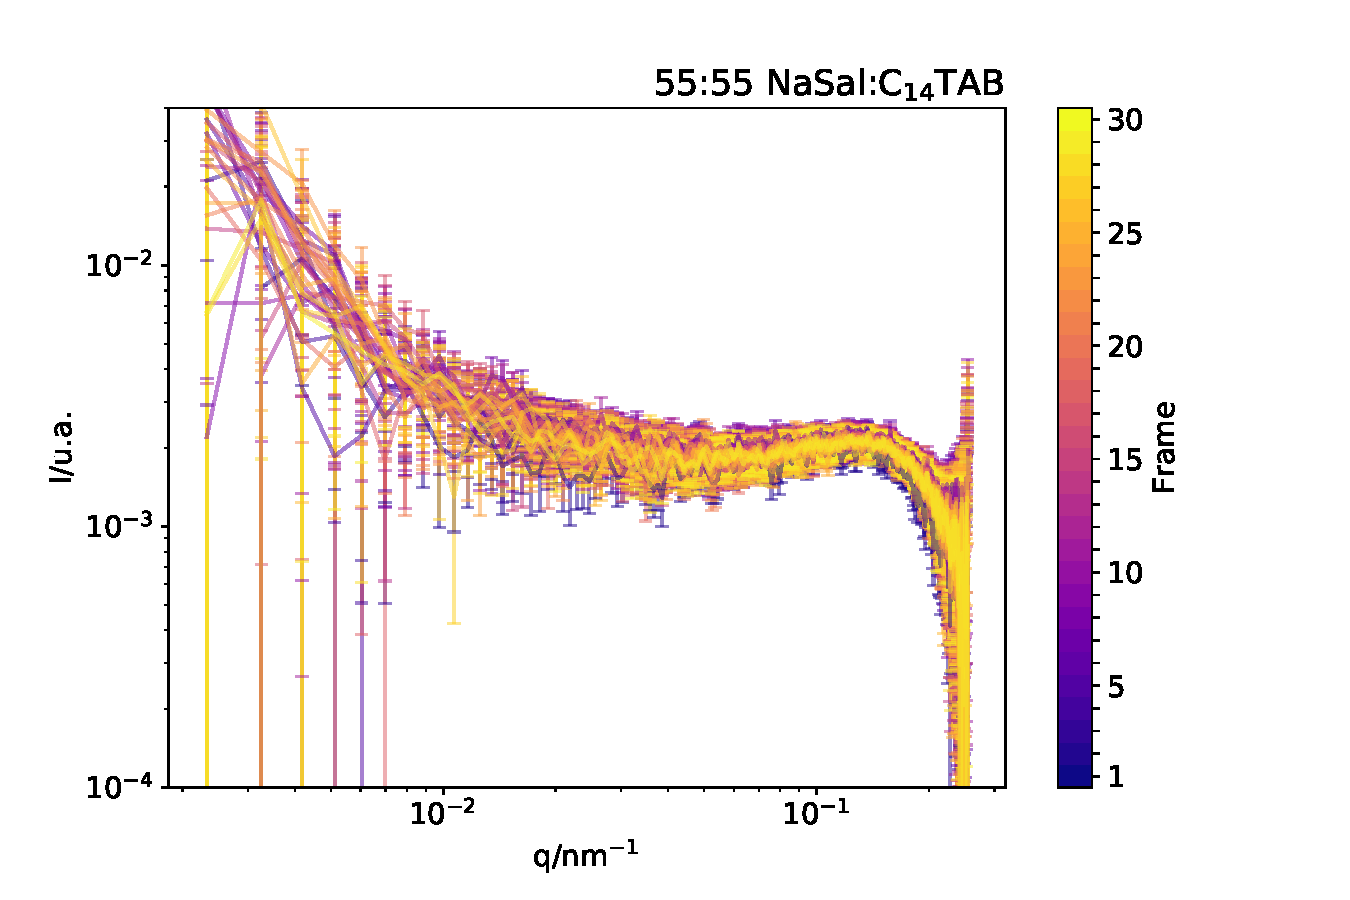
\includegraphics[width=\textwidth]{imagens/saxs/TR_saxs_55_55_dados.pdf}
			\caption{Dados}
			\label{fig:saxs_tr_55_d}
		\end{subfigure}%
		\begin{subfigure}[t]{0.5\textwidth}
			\centering
			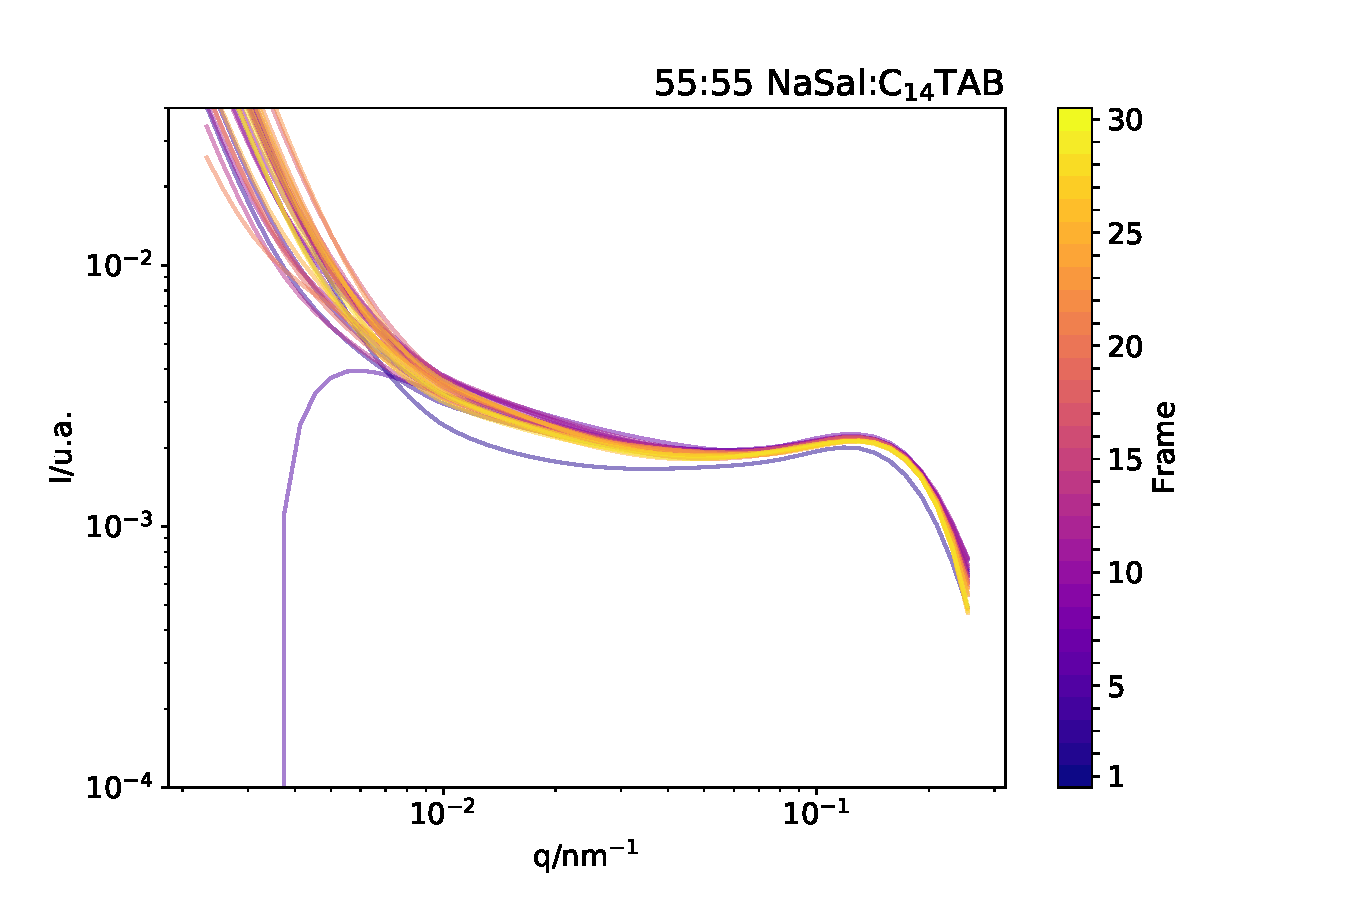
\includegraphics[width=\textwidth]{imagens/saxs/TR_saxs_55_55_ajuste.pdf}
			\caption{Ajustes}
			\label{fig:saxs_tr_55_a}
		\end{subfigure}
		\caption{Dados experimentais médios das curvas de SAXS nas aquisições numeradas de 1-30, numeradas do menor ao maior tempo de espera. As curvas foram obtidas pela mistura de 55 \mM{} de NaSal com 55\mM{} de \TTAB.}
		\label{fig:saxs_tr_55}
	\end{figure} 

	\begin{figure}[h]
		\begin{subfigure}[t]{0.5\textwidth}
			\centering
			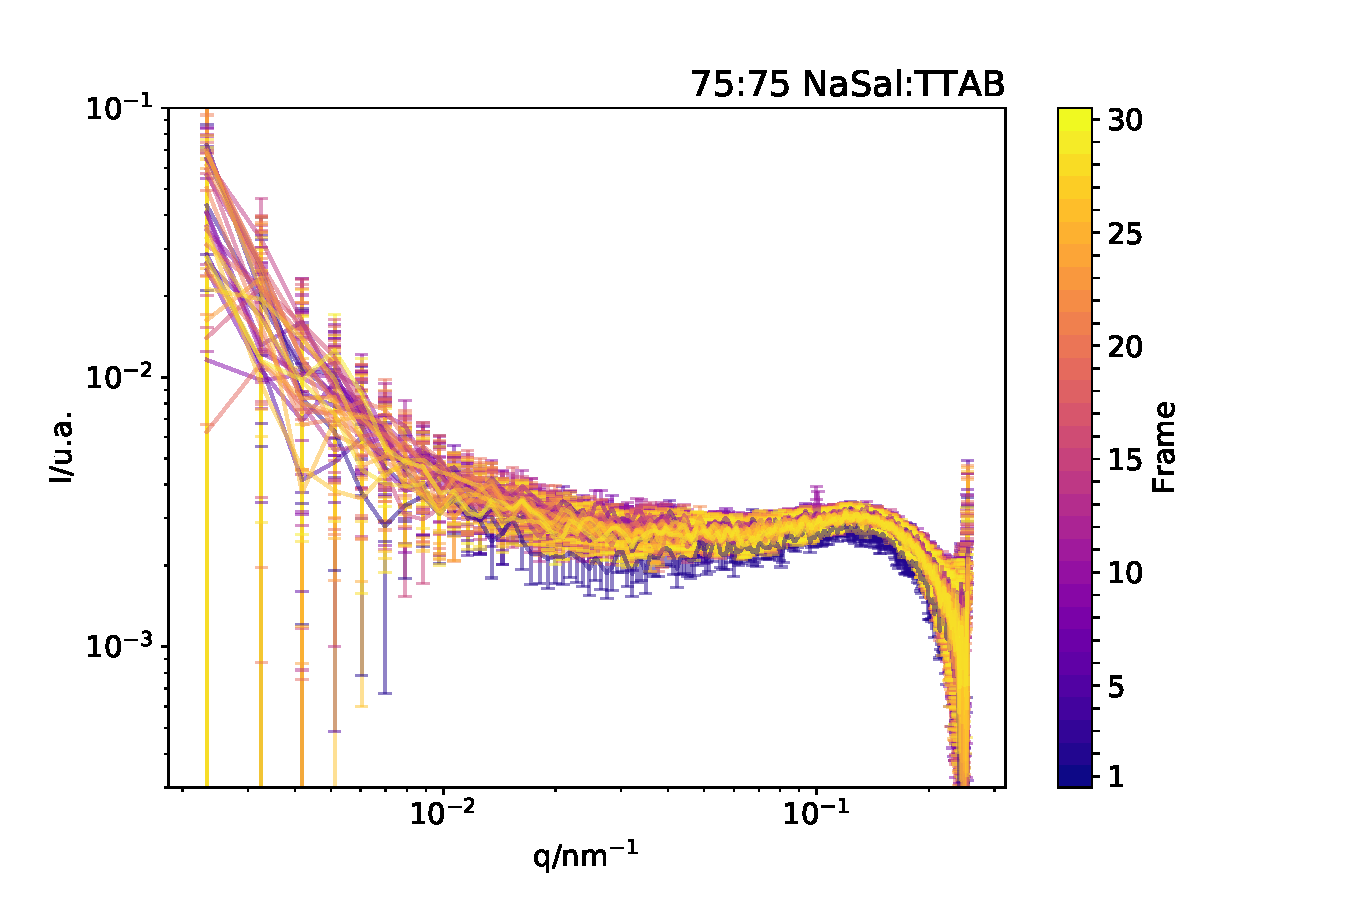
\includegraphics[width=\textwidth]{imagens/saxs/TR_saxs_75_75_dados.pdf}
			\caption{Dados}
			\label{fig:saxs_tr_75_d}
		\end{subfigure}%
		\begin{subfigure}[t]{0.5\textwidth}
			\centering
			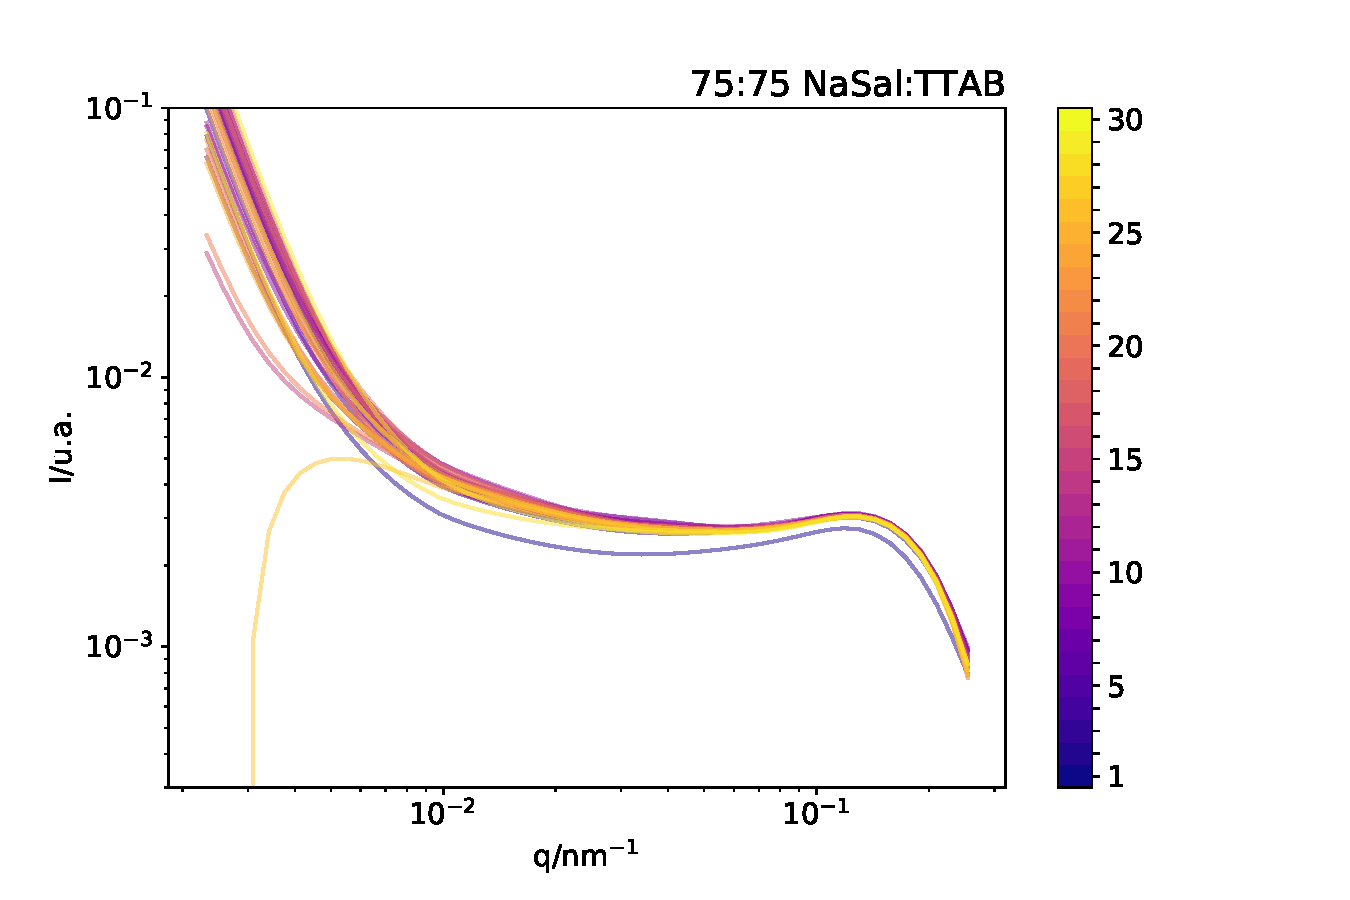
\includegraphics[width=\textwidth]{imagens/saxs/TR_saxs_75_75_ajuste.pdf}
			\caption{Ajustes}
			\label{fig:saxs_tr_a}
		\end{subfigure}
		\caption{Dados experimentais médios das curvas de SAXS nas aquisições numeradas de 1-30, numeradas do menor ao maior tempo de espera. As curvas foram obtidas pela mistura de 75 \mM{} de NaSal com 75 \mM{} de \TTAB.}
		\label{fig:saxs_tr_75}
	\end{figure} 
	
	\begin{figure}[h]
		\begin{subfigure}[t]{0.5\textwidth}
			\centering
			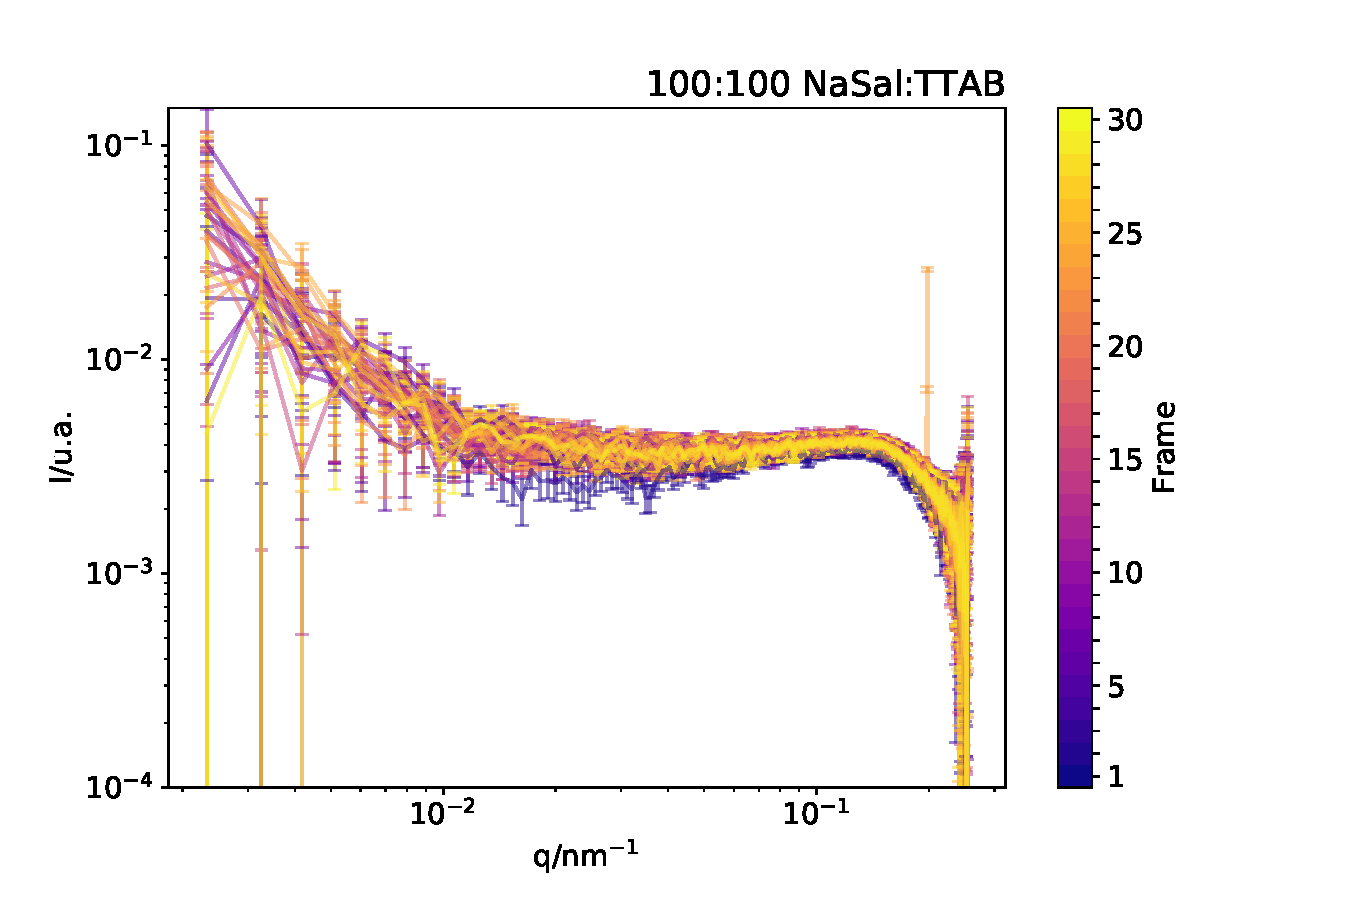
\includegraphics[width=\textwidth]{imagens/saxs/TR_saxs_100_100_dados.pdf}
			\caption{Dados}
			\label{fig:saxs_tr_100_d}
		\end{subfigure}%
		\begin{subfigure}[t]{0.5\textwidth}
			\centering
			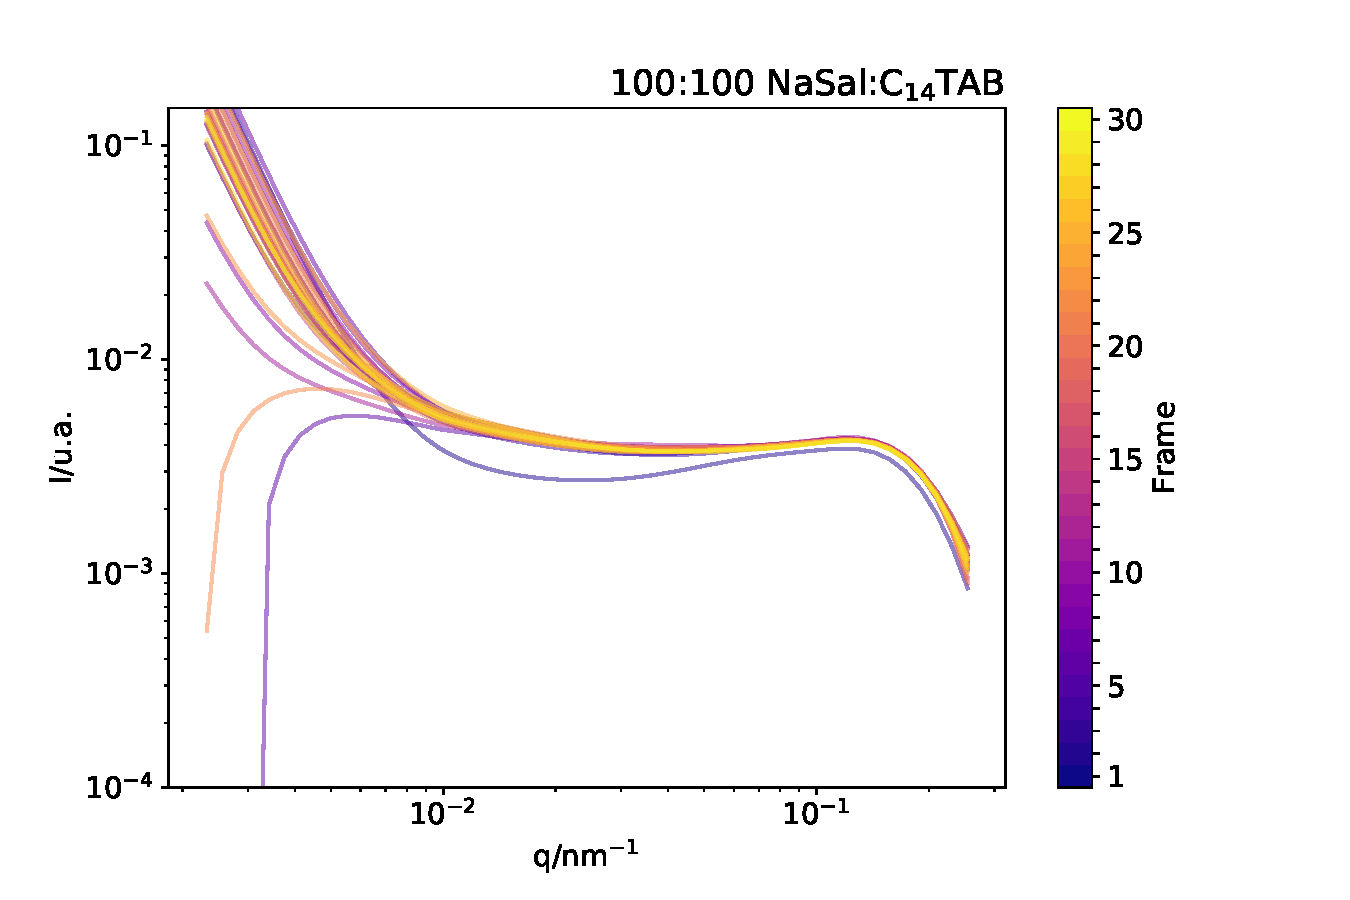
\includegraphics[width=\textwidth]{imagens/saxs/TR_saxs_100_100_ajustes.pdf}
			\caption{Ajustes}
			\label{fig:saxs_tr_100_a}
		\end{subfigure}
		\caption{Dados experimentais médios das curvas de SAXS nas aquisições numeradas de 1-30, numeradas do menor ao maior tempo de espera. As curvas foram obtidas pela mistura de 100 \mM{} de NaSal com 100 \mM{} de \TTAB.}
		\label{fig:saxs_tr_100}
	\end{figure} 
	
	\begin{figure}[h]
		\begin{subfigure}[t]{0.5\textwidth}
			\centering
			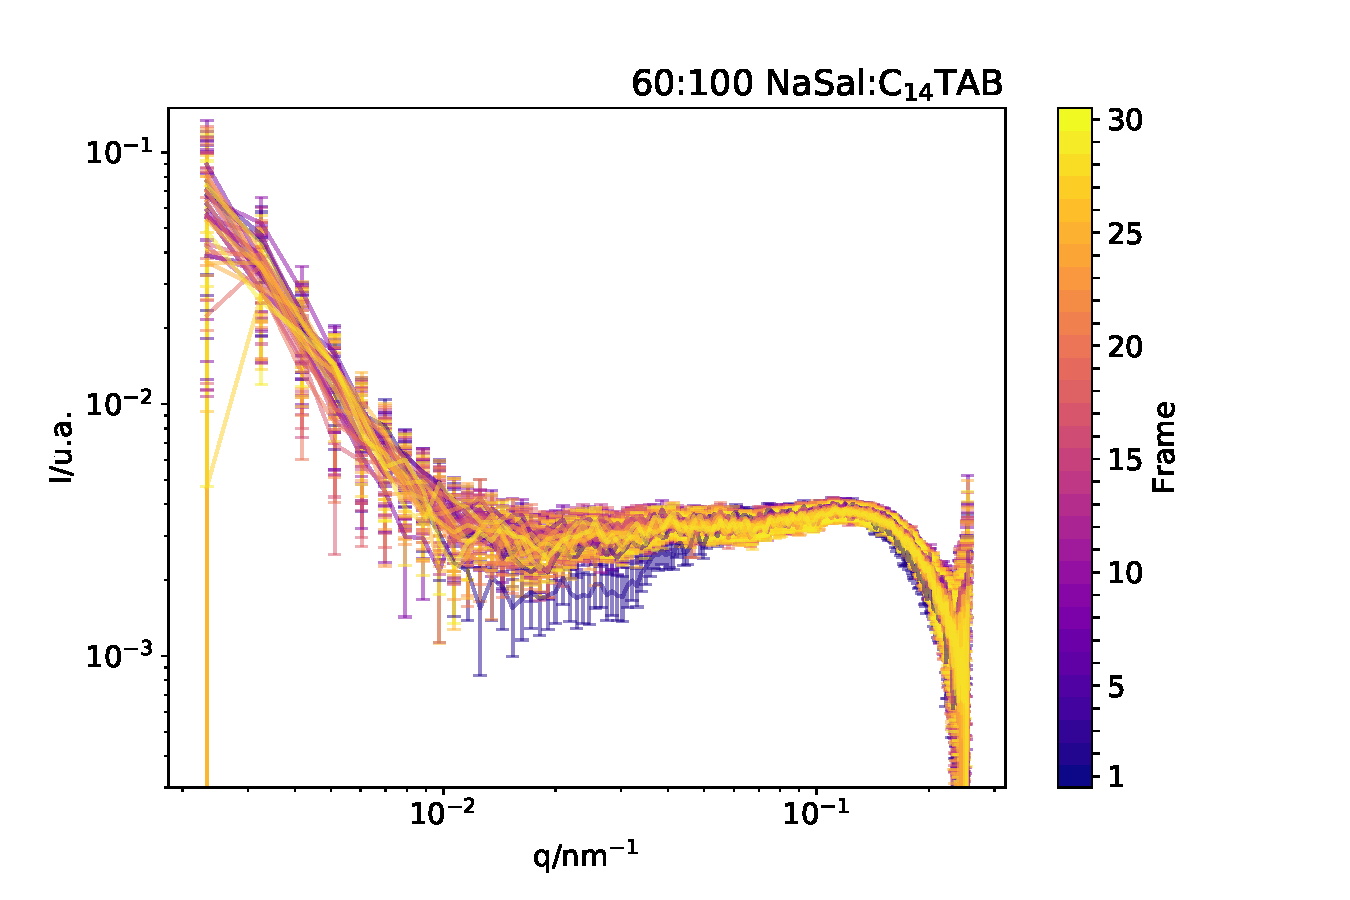
\includegraphics[width=\textwidth]{imagens/saxs/TR_saxs_60_100_3_dados.pdf}
			\caption{Dados}
			\label{fig:saxs_tr_60_3_d}
		\end{subfigure}%
		\begin{subfigure}[t]{0.5\textwidth}
			\centering
			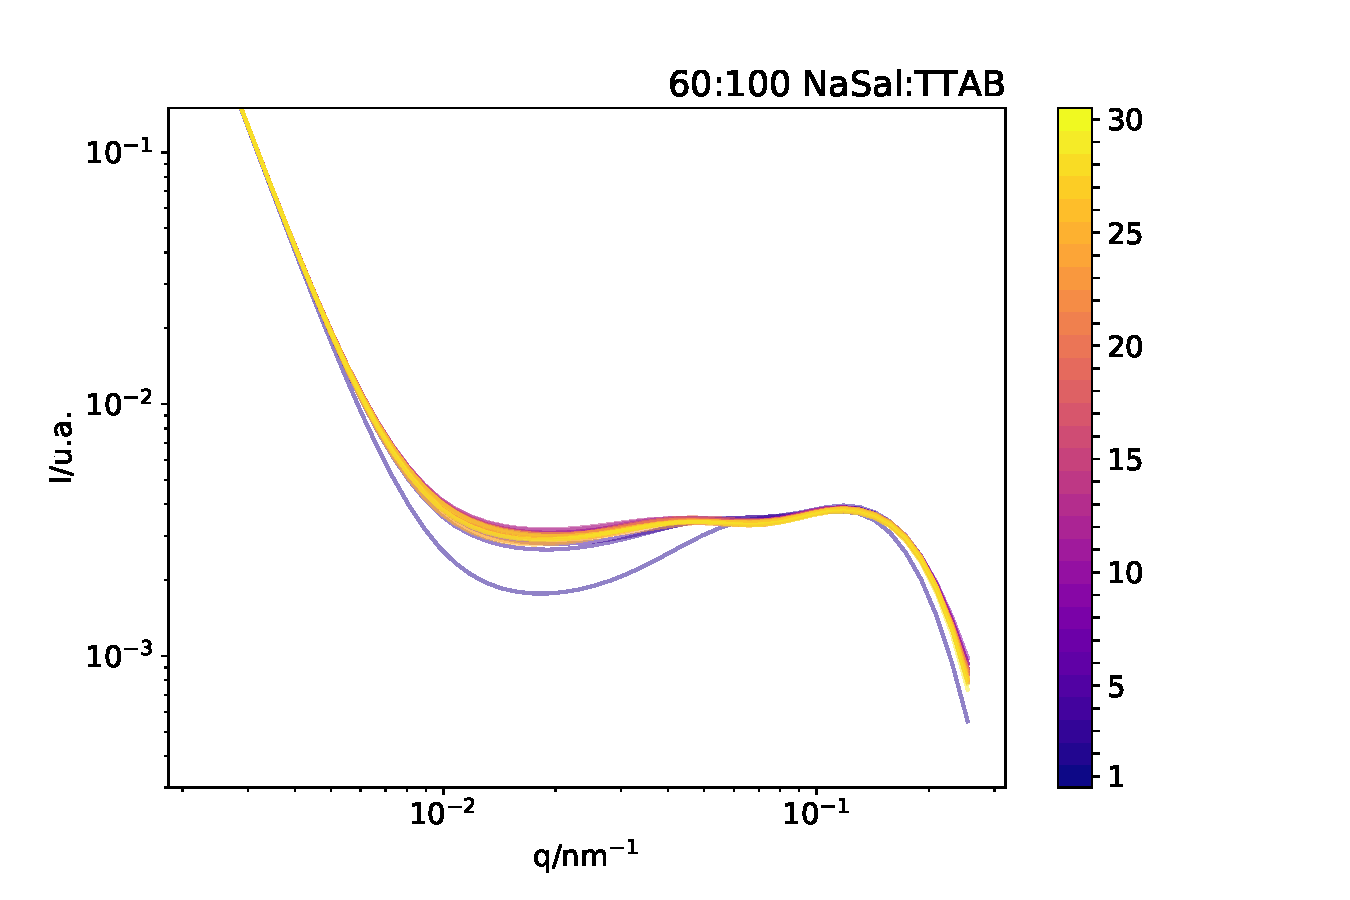
\includegraphics[width=\textwidth]{imagens/saxs/TR_saxs_60_100_3_ajustes.pdf}
			\caption{Ajustes}
			\label{fig:saxs_tr_60_3_a}
		\end{subfigure}
		\caption{Dados experimentais médios das curvas de SAXS nas aquisições numeradas de 1-30, numeradas do menor ao maior tempo de espera. As curvas foram obtidas pela mistura de 60 \mM{} de NaSal com 100 \mM{} de \TTAB.}
		\label{fig:saxs_tr_60_3}
	\end{figure} 

	\begin{figure}[h]
		\begin{subfigure}[t]{0.5\textwidth}
			\centering
			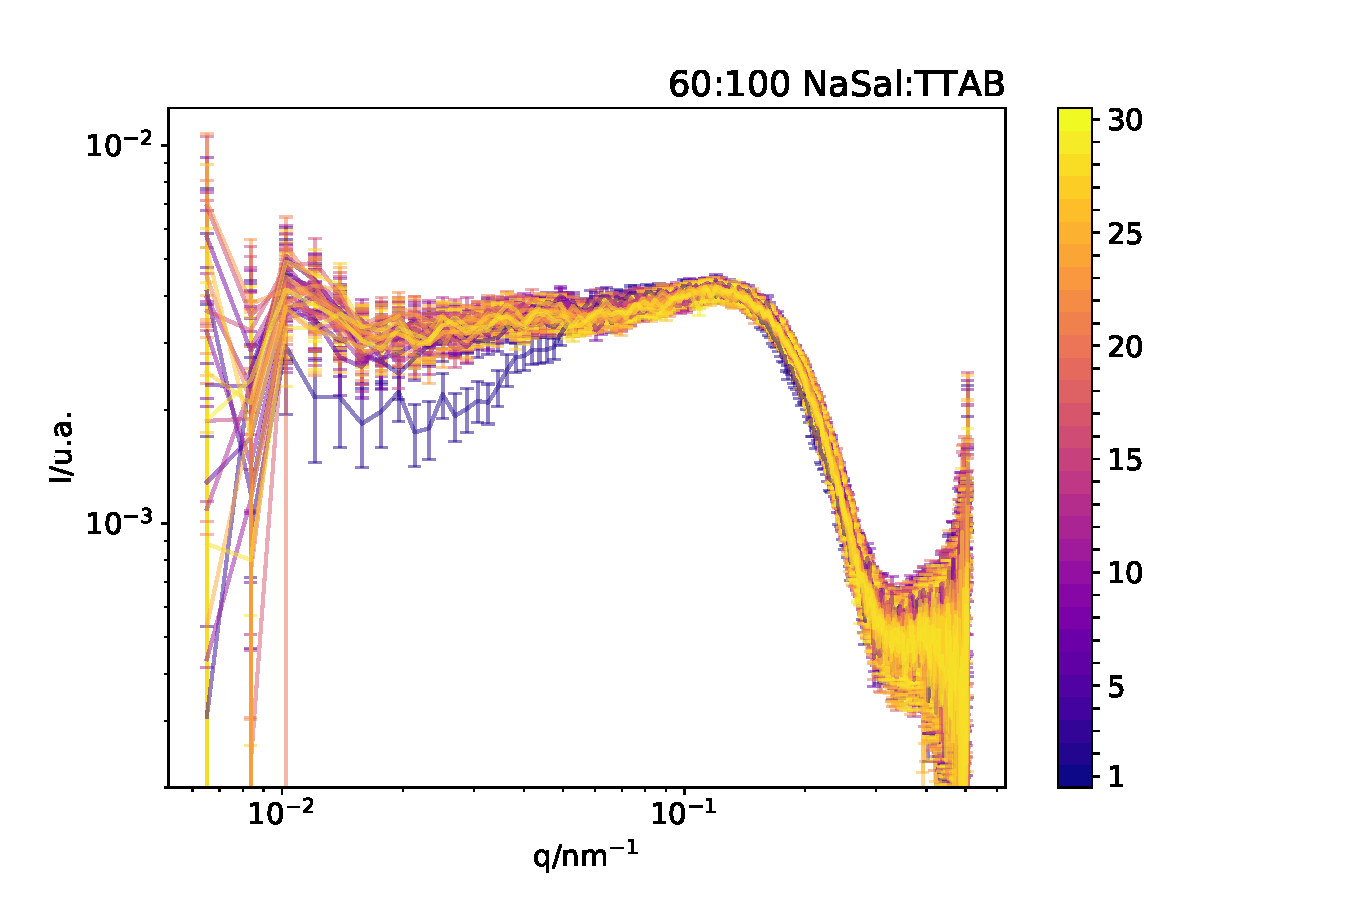
\includegraphics[width=\textwidth]{imagens/saxs/TR_saxs_60_100_15_dados.pdf}
			\caption{Dados}
			\label{fig:saxs_tr_60_15_d}
		\end{subfigure}%
		\begin{subfigure}[t]{0.5\textwidth}
			\centering
			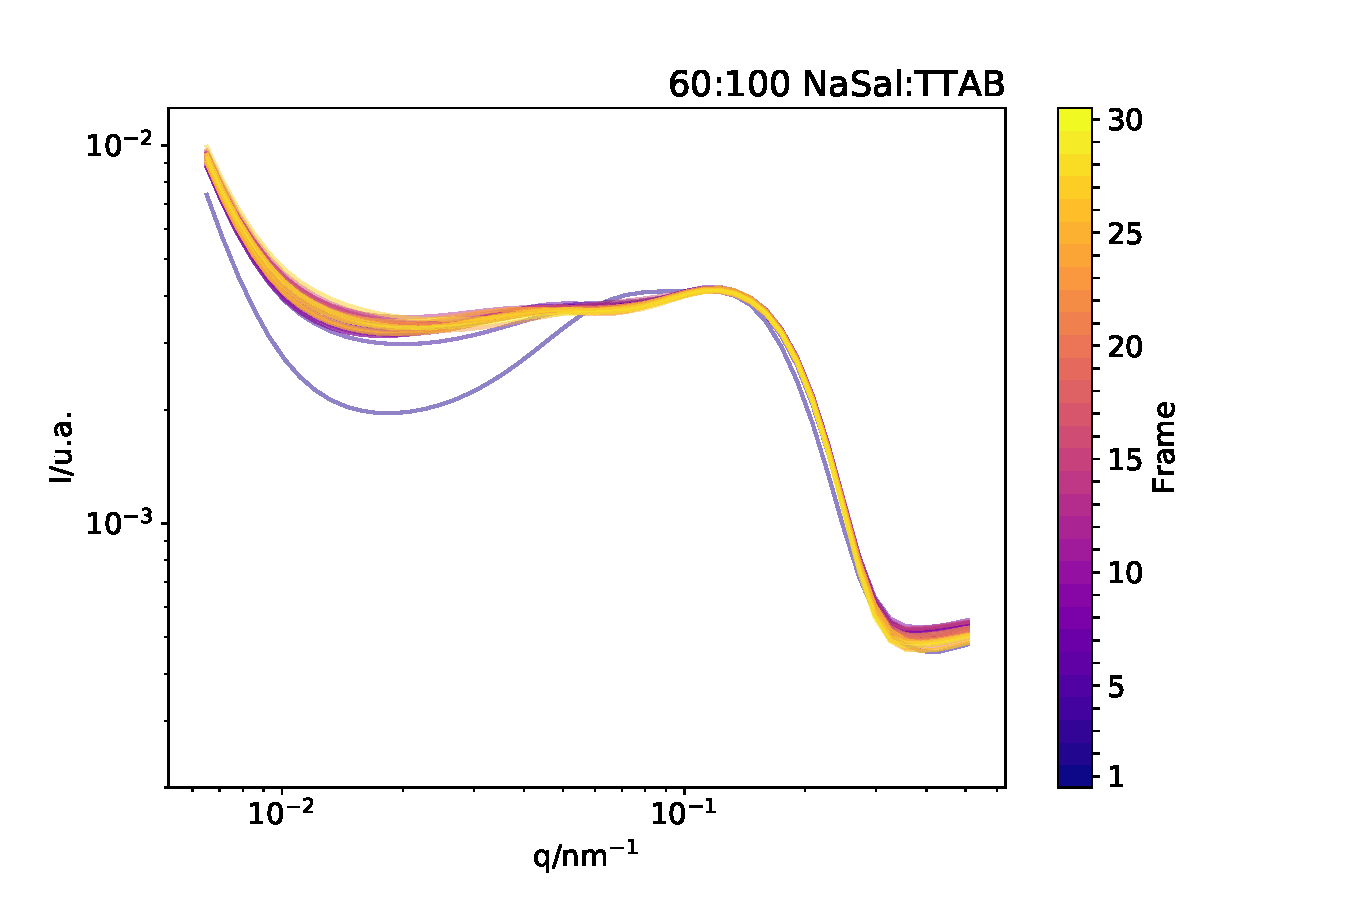
\includegraphics[width=\textwidth]{imagens/saxs/TR_saxs_60_100_15_ajustes.pdf}
			\caption{Ajustes}
			\label{fig:saxs_tr_60_15_a}
		\end{subfigure}
		\caption{Dados experimentais médios das curvas de SAXS nas aquisições numeradas de 1-30, numeradas do menor ao maior tempo de espera. As curvas foram obtidas pela mistura de 60 \mM{} de NaSal com 60 \mM{} de \TTAB. Neste caso, a distância do detector é de 1,5m, abrangendo uma faixa de \q{} diferente.}
		\label{fig:saxs_tr_60_15}
	\end{figure} 
	
%	\FloatBarrier
	
	Todos os primeiros \emph{frames} das curvas possuem um formato diferente dos demais, que é mais pronunciado à medida que a concentração aumenta. Isso mostra que em 35 ms, as micelas possuíam uma estrutura diferente do que em 65 ms, e adiante. Essas curvas são, todavia, bastante próximas em formato ao estado final da \autoref{fig:tr_comparacao_ttab}, o que significa que o crescimento micelar está quase completo em 35 ms e se completa em 65 ms. Uma possível explicação para esse acontecimento é a alta concentração de micelas no meio. Isso acelera a cinética de colisão entre micelas e cossolutos. Além disso, a rede micelar pode se tornar tão densa que o meio se torna homogêneo para SAXS, e não é possível distinguir entre uma micela e outra.
	
	Na maior parte das curvas, é possível observar que na região de baixo \q, há um decaimento exponencial. O modelo utilizado não prevê esse comportamento, que teve de ser incluído externamente. O valor do expoente, em todos os ajustes, foi de 4, isto é, o decaimento segue \( q^{-4} \). Se essa região for verdadeira, a validade do modelo utilizado para o tratamento se torna questionável. Porém, essa queda não foi observada na cela de \emph{flow-through}, como mencionado anteriormente. Além disso, houveram ligeiras variações no valor do \emph{background} entre cada amostra, devido à limpeza, apesar de que se garantiu que nenhum sinal significativo era observado. A \autoref{fig:problema_limpeza} mostra a minúscula diferença entre o \emph{background}, medido com o capilar seco e vazio, e o capilar após a primeira limpeza com água. Essa pequena diferença pode gerar o sinal em baixo \q{} com o decaimento observado devido à baixa intensidade nos sinais, devido ao curto tempo de integração, necessário para medidas cinéticas, e o baixo contraste entre as micelas e o solvente. Logo, a região em baixo \q{}, provavelmente, não possui significado físico, e o decaimento exponencial utilizado é somente um artifício matemático para auxiliar no ajuste das curvas.
	
	\begin{figure}[h]
		\centering
		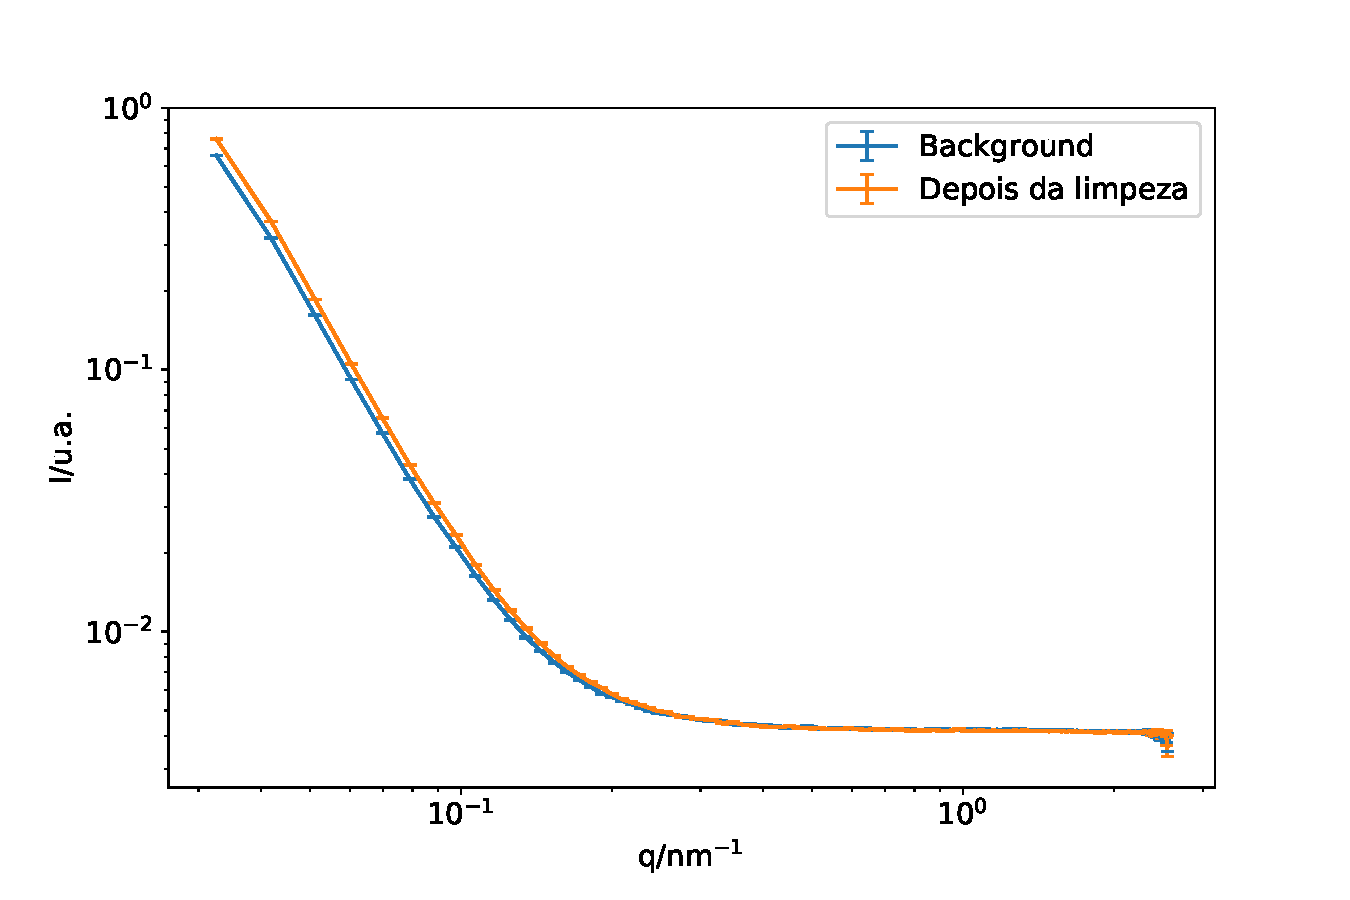
\includegraphics[width=0.7\textwidth]{imagens/saxs/problema_limpeza}
		\caption{Diferença entre o sinal de SAXS do \emph{background} e após a limpeza com água.}
		\label{fig:problema_limpeza}
	\end{figure}

	Os resultados dos ajustes se encontram nas Figuras \ref{fig:params_dhead_radcore}, \ref{fig:params_nurpa_dcq} e \ref{fig:params_scale_rhorel}. A \autoref{tab:params_ajuste_saxs} resume as mesmas informações. Parte dos parâmetros de ajuste não foram variados, para auxiliar na convergência. Por exemplo, o comprimento de Kuhn e de contorno foram fixados em 1000 nm e 5000 nm, respectivamente, pois a alteração de qualquer um não resultava numa alteração significativa das curvas. Isso significa que não foi possível observar a cinética de mudança do comprimento das micelas por essa técnica. As diferenças nos formatos das curvas se devem a outros parâmetros.
			
	\begin{figure}
		\begin{subfigure}[t]{0.5\textwidth}
			\centering
			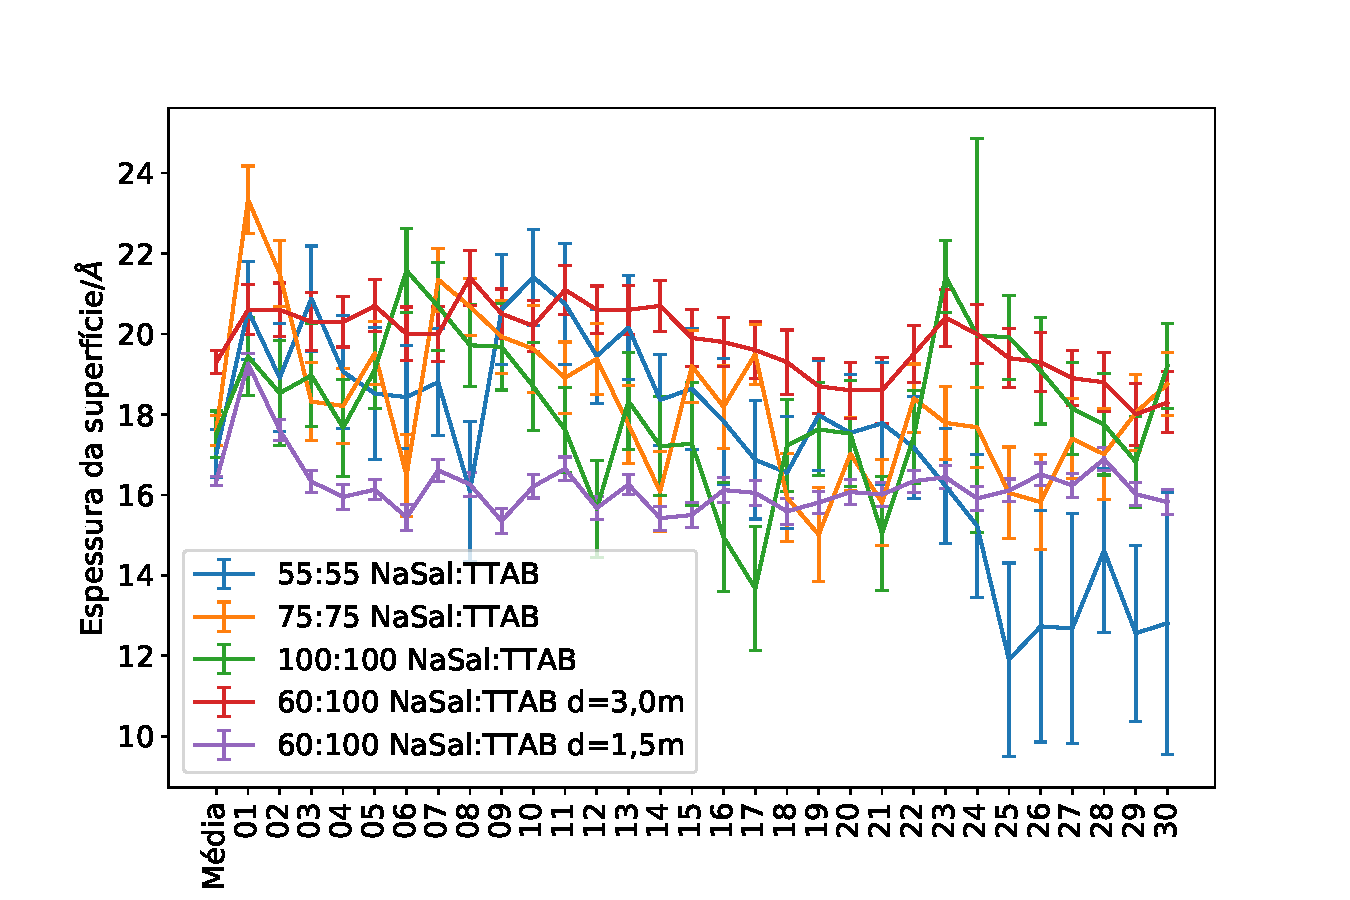
\includegraphics[width=\textwidth]{imagens/saxs/param_d_head}
			\caption{Espessura da superfície, \(d_{\mathrm{head}}\)}
			\label{fig:param_dhead}
		\end{subfigure} %
		\begin{subfigure}[t]{0.5\textwidth}
			\centering
			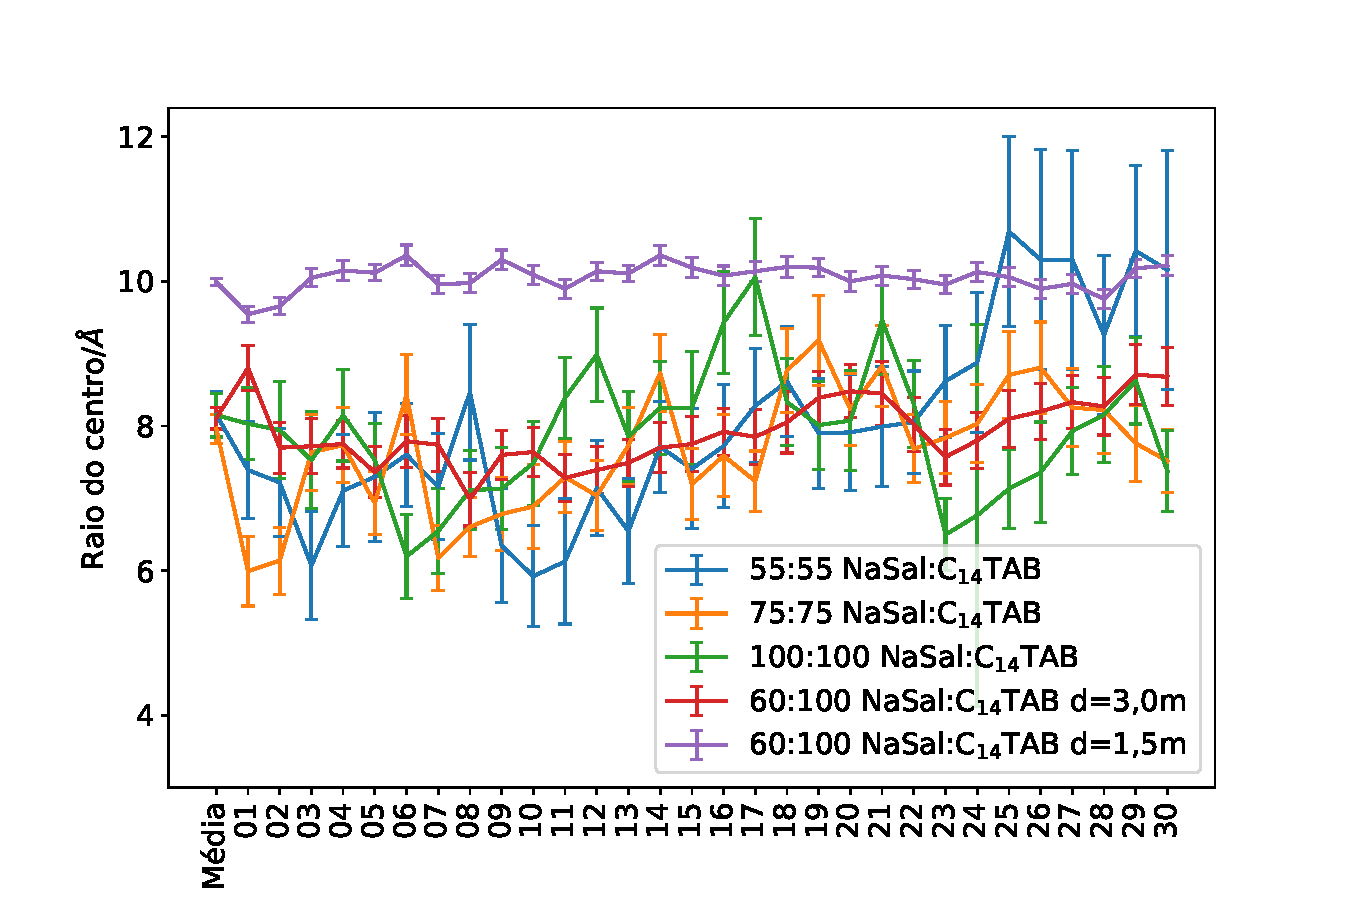
\includegraphics[width=\textwidth]{imagens/saxs/param_rad_core}
			\caption{Raio do centro, \(r_{\mathrm{core}}\)}
			\label{fig:param_radcore}
		\end{subfigure}
		\caption{Parâmetros \(d_{\mathrm{head}}\) e \(r_{\mathrm{core}}\), ambos em \AA, das cinco amostras medidas. Os números indicam o \emph{frame}, e o tempo após a mistura pode ser checada na \autoref{tab:tr_tempos_frames}. ``Média'' significa o resultado do ajuste da média das curvas 2-30, que eram praticamente idênticas.}
		\label{fig:params_dhead_radcore}
	\end{figure} \index{resultados!SAXS!ajustes}

	\begin{figure}
		\begin{subfigure}[t]{0.5\textwidth}
			\centering
			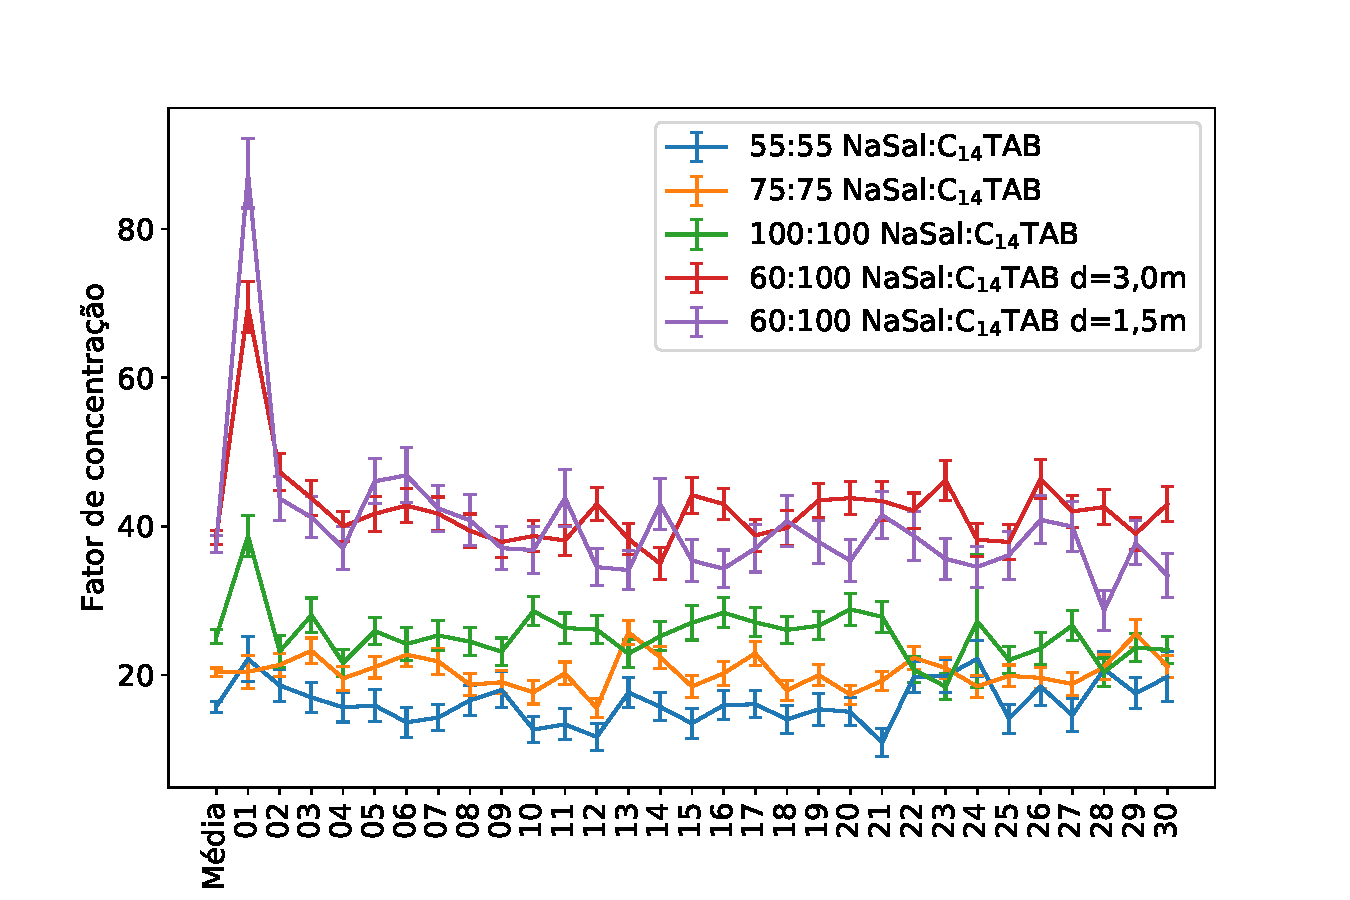
\includegraphics[width=\textwidth]{imagens/saxs/param_nu_rpa}
			\caption{Fator de concentração \(\nu_{\mathrm{RPA}}\)}
			\label{fig:param_nurpa}
		\end{subfigure} %
		\begin{subfigure}[t]{0.5\textwidth}
			\centering
			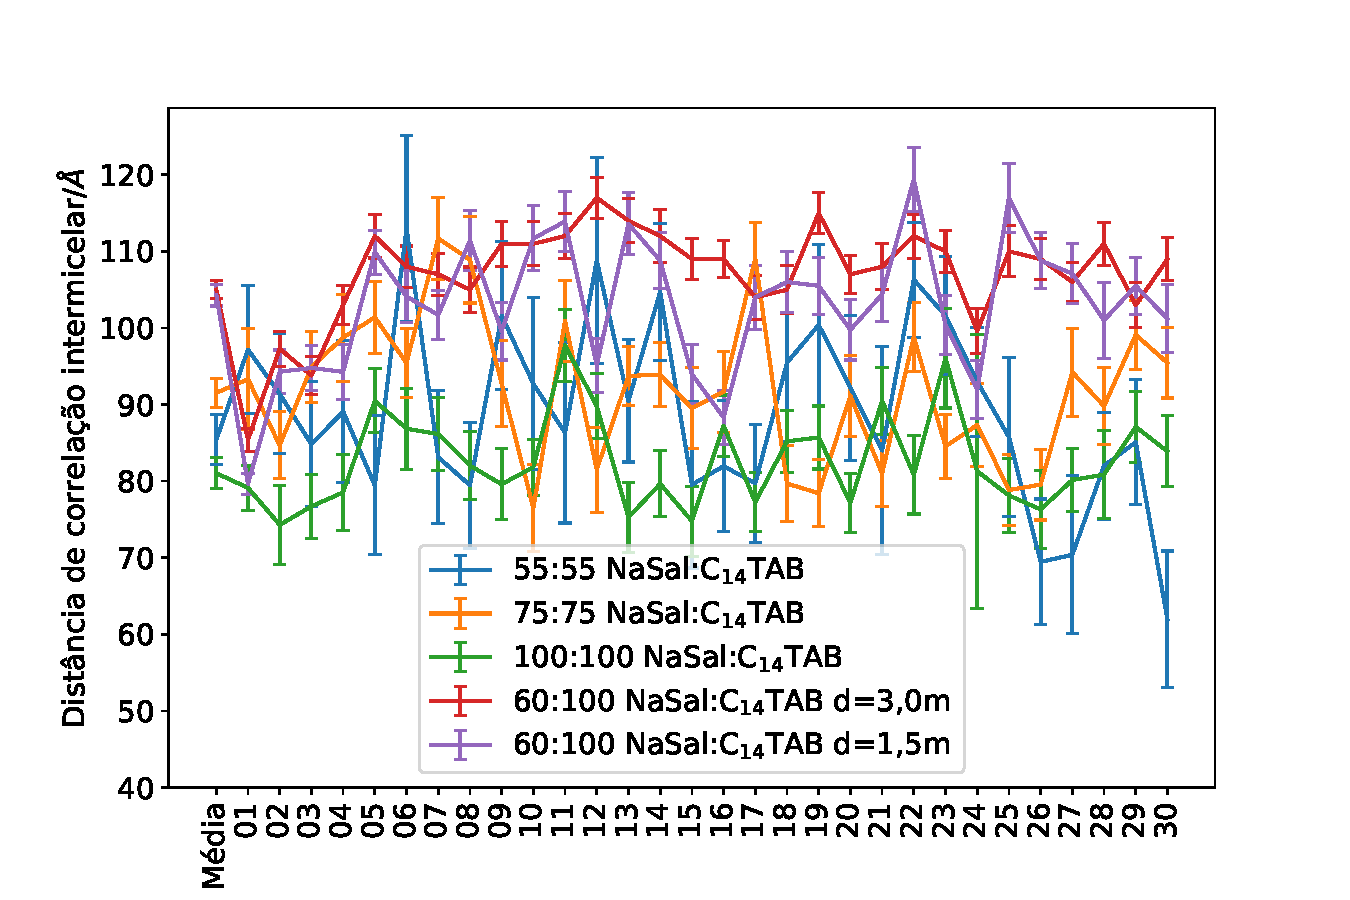
\includegraphics[width=\textwidth]{imagens/saxs/param_d_cq}
			\caption{Distância de correlação \(D_{\mathrm{cq}}\)}
			\label{fig:param_dcq}
		\end{subfigure}
		\caption{Parâmetros \(\nu_{\mathrm{RPA}}\) e \(D_{\mathrm{cq}}\) em \AA, das cinco amostras medidas. Os números indicam o \emph{frame}, e o tempo após a mistura pode ser checada na \autoref{tab:tr_tempos_frames}. ``Média'' significa o resultado do ajuste da média das curvas 2-30, que eram praticamente idênticas.}
		\label{fig:params_nurpa_dcq}
	\end{figure}

	\begin{figure}
		\begin{subfigure}[t]{0.5\textwidth}
			\centering
			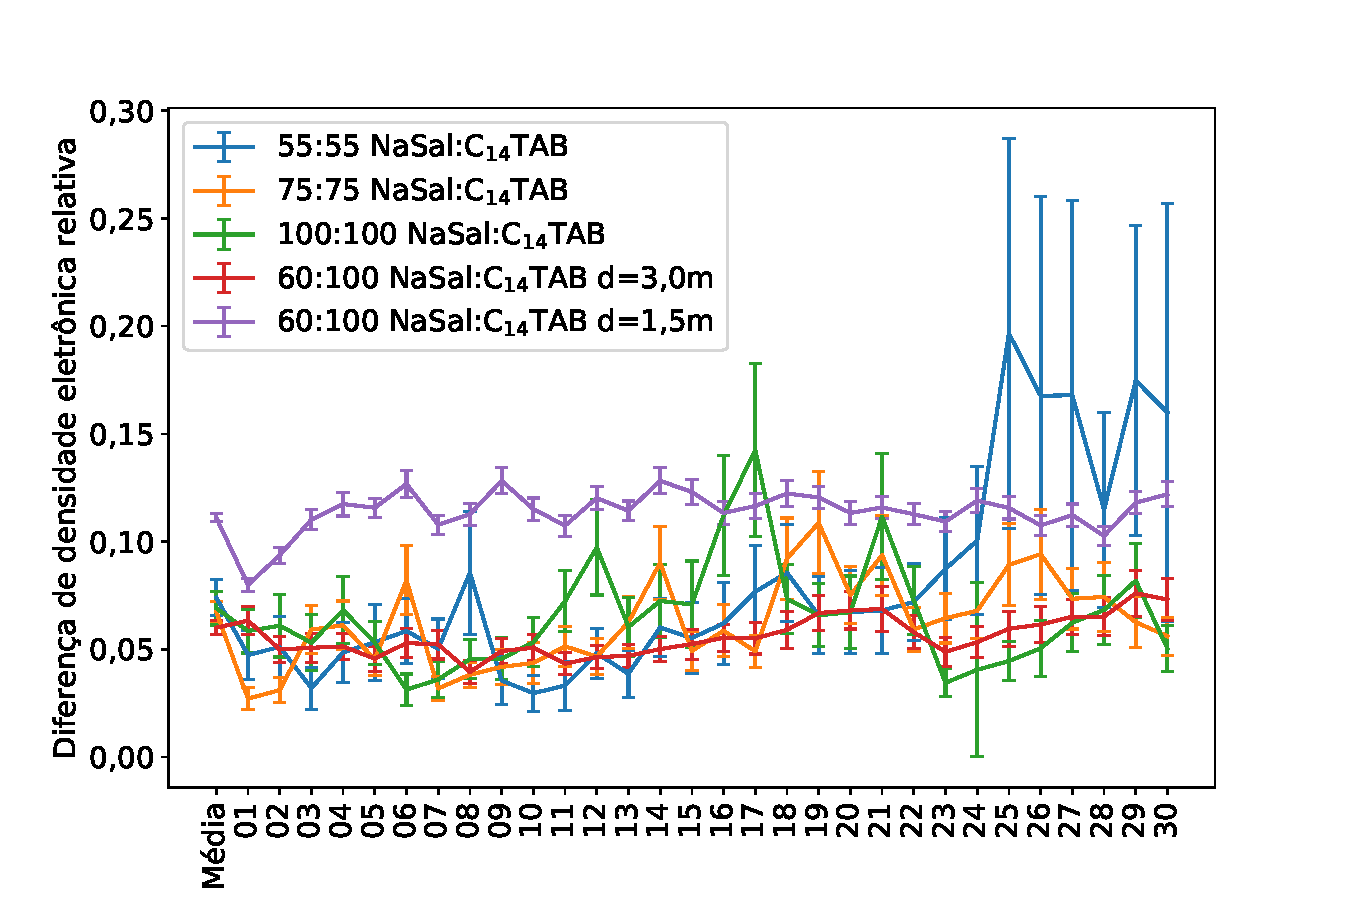
\includegraphics[width=\textwidth]{imagens/saxs/param_rho_rel}
			\caption{Diferença de densidade eletrônica relativa \(\rho_{\mathrm{rel}}\)}
			\label{fig:param_rhorel}
		\end{subfigure} %
		\begin{subfigure}[t]{0.5\textwidth}
			\centering
			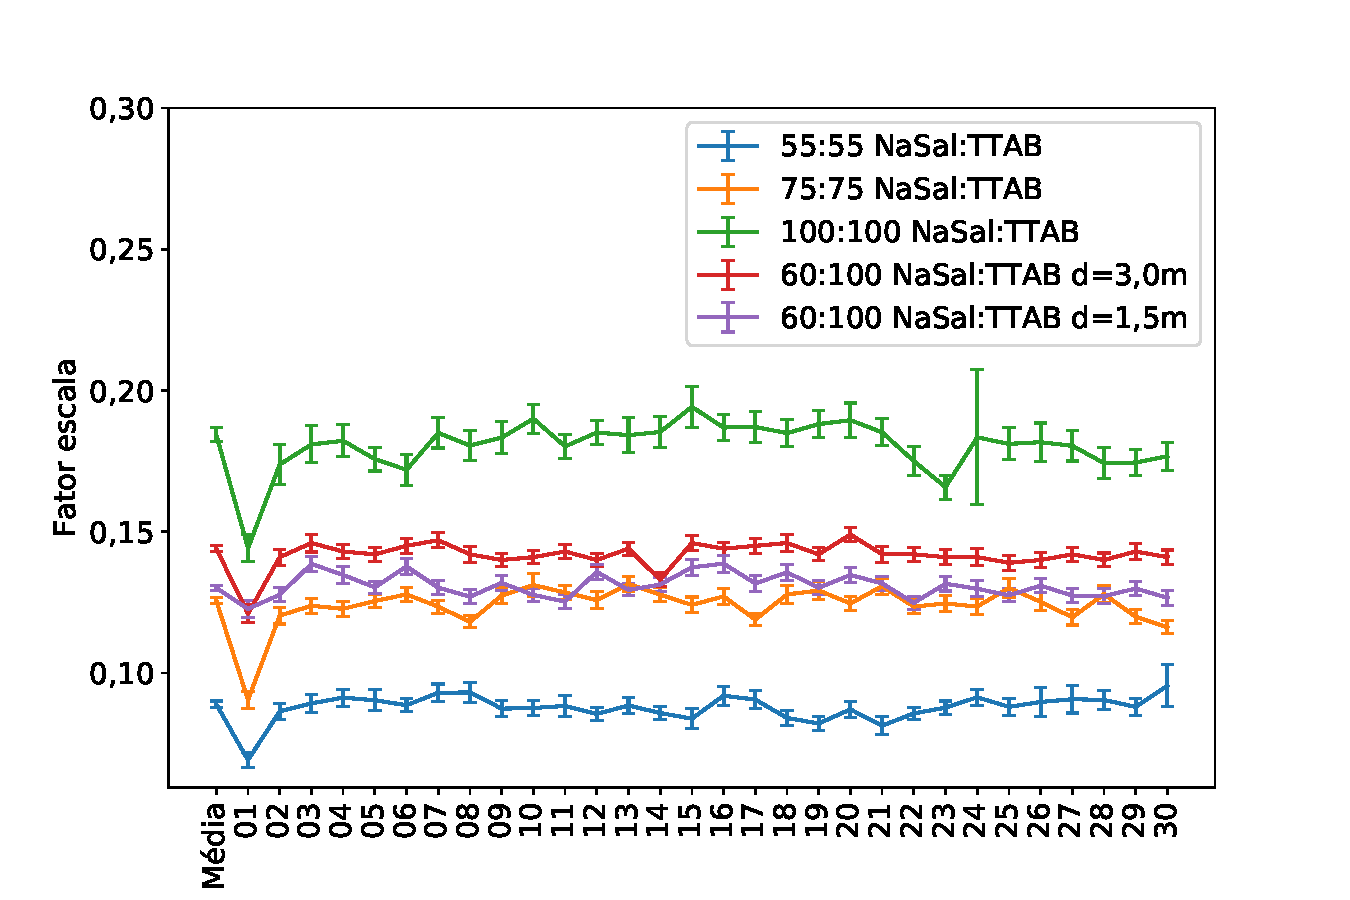
\includegraphics[width=\textwidth]{imagens/saxs/param_scale}
			\caption{Fator de escala}
			\label{fig:param_scale}
		\end{subfigure}
		\caption{Parâmetros \(\rho_{\mathrm{rel}}\) e \(\mathrm{scale}\) das cinco amostras medidas. Os números indicam o \emph{frame}, e o tempo após a mistura pode ser checada na \autoref{tab:tr_tempos_frames}. ``Média'' significa o resultado do ajuste da média das curvas 2-30, que eram praticamente idênticas.}
		\label{fig:params_scale_rhorel}
	\end{figure}

	
	\begin{table}[h]
		\IBGEtab{%
			\caption{Parâmetros de ajuste das curvas de SAXS escolhidos para comparação. Como as curvas 2--30 são praticamente idênticas, foi realizada uma média delas, que depois foi ajustada ao modelo, resultando nos parâmetros aqui.}
			\label{tab:params_ajuste_saxs}
		}%
		{%
			\begin{tabular}{c c | c c c c c c}
				\toprule
				            Composição             & Posição  & \(\mathrm{scale}\)/\(10^3\) & \(d_{\mathrm{head}}\)/\AA    & \(r_{\mathrm{core}}\)/\AA       & \(\rho_{\mathrm{rel}}\)   & \(D_{CQ}\)\AA & \(\nu_{RPA}\)      \\ \midrule
				   \multirow{2}{*}{55:55}    & Média    & 89  \(\pm\) 1   & 17,0   \(\pm\) 0,6 & 8,2      \(\pm\) 0,3  & 74   \(\pm\)  8  & 85 \(\pm\) 3  & 15,8   \(\pm\) 0,7 \\
				                             & Primeiro & 69  \(\pm\) 3   & 21   \(\pm\) 1     & 7,4      \(\pm\) 0,7  & 50    \(\pm\) 10 & 97 \(\pm\) 8  & 22,0   \(\pm\) 3,0 \\
				   \multirow{2}{*}{75:75}    & Média    & 126  \(\pm\) 1  & 17,6   \(\pm\) 0,4 & 8,0      \(\pm\) 0,2  & 67   \(\pm\)  5  & 92 \(\pm\) 2  & 20,4   \(\pm\) 0,6 \\
				                             & Primeiro & 90  \(\pm\) 3   & 23,3   \(\pm\) 0,8 & 6,0      \(\pm\) 0,5  & 27   \(\pm\)  5  & 93 \(\pm\) 7  & 20,0   \(\pm\) 2,0 \\
				  \multirow{2}{*}{100:100}   & Média    & 184  \(\pm\) 3  & 17,5   \(\pm\) 0,6 & 8,2      \(\pm\) 0,3  & 69   \(\pm\)  8  & 81 \(\pm\) 2  & 25,2   \(\pm\) 0,9 \\
				                             & Primeiro & 144  \(\pm\) 5  & 19   \(\pm\) 1     & 8,0      \(\pm\) 0,5  & 60    \(\pm\) 10 & 79 \(\pm\) 3  & 39,0   \(\pm\) 3,0 \\
				  \multirow{2}{*}{60:100}    & Média    & 144  \(\pm\) 1  & 19,3   \(\pm\) 0,3 & 8,1      \(\pm\) 0,2  & 60    \(\pm\) 3  & 105 \(\pm\) 1 & 38,5   \(\pm\) 0,9 \\
				                             & Primeiro & 121  \(\pm\) 3  & 20,6   \(\pm\) 0,6 & 8,8      \(\pm\) 0,3  & 63   \(\pm\)  6  & 85 \(\pm\) 1  & 70,0   \(\pm\) 3,0 \\
				\multirow{2}{*}{60:100 1,5m} & Média    & 130  \(\pm\) 1  & 16,4   \(\pm\) 0,1 & 9,99     \(\pm\) 0,05 & 111   \(\pm\)  2 & 104 \(\pm\) 1 & 38,0   \(\pm\) 1   \\
				                             & Primeiro & 123  \(\pm\) 3  & 19,3   \(\pm\) 0,3 & 9,5      \(\pm\) 0,1  & 80    \(\pm\) 3  & 80 \(\pm\) 1  & 87   \(\pm\) 5     \\ \bottomrule
			\end{tabular}
		}{}
	\end{table} 

	Os parâmetros obtidos da amostra 60:100 NaSal:TTAB nas duas distâncias de detector são, em alguns casos, diferentes. Isso ocorre nas medidas da espessura da superfície, raio do \emph{core}, e na diferença de densidade eletrônica. O raio do \emph{core} e da superfície são complementares, e aparecem na região de alto \q, devido ao pequeno tamanho. Logo, as amostras com d=1,5 m, que possuem melhor definição na região de alto \q, também possuem barras de erro menores, em ambos \(r_{\mathrm{core}}\) e \(d_{\mathrm{head}}\). Além disso, os valores de \(r_{\mathrm{core}}\) são maiores para d=1,5 m, mas \(d_\mathrm{head}\) são complementarmente menores. De qualquer maneira, ambas as distâncias são bastante semelhantes em todas as amostras. Interessantemente, o valor médio da primeira medida é consistentemente diferente das outras, resultado do crescimento das micelas entre o primeiro e os próximos \emph{frames}.
	
	O comprimento da cadeia de surfactante pode ser estimado pela equação de Tanford (\autoref{eqn:tanford}). Com isso, o raio de seção transversal de micelas gigantes com \TTAB{} (\(n=14\)) é de aproximadamente 2 nm, ou 20 \AA. Considerando a presença do grupo trimetilamônio, carregado, e da molécula de salicilato, que pode se posicionar na paliçada micelar próximo à superfície ou mais no interior, os tamanhos calculados para \(d_{\mathrm{head}}\) e \(r_{\mathrm{core}}\) são factíveis, com um raio total de 30 \AA{} (3 nm).

	A diferença entre o primeiro e os últimos \emph{frames} também foi observada no fator de concentração e na distância de correlação. Quanto maior a concentração, maior foi o efeito, e foi máximo no caso onde a composição é 60:100. A diferença entre o primeiro e os últimos frames do fator de concentração pode se dever, ao crescimento das micelas. Antes do crescimento estar finalizado, não há uma rede micelar tão densa, então o fator de concentração é diferente. A distância de correlação, pelo outro lado, mostra que antes do crescimento, a carga superficial micelar era menor, devido à menor distância, e depois se estabilizou. Essas propriedades foram as mais importantes para a diferenciação entre o primeiro \emph{frame} e os demais.
	
	Por último, vemos que a maior parte das amostras possui o parâmetro \(\rho_{\mathrm{rel}}\) próximos, com o caso 60:100 1,5 m sendo o mais discrepante. Há uma diferença entre o primeiro e os últimos \emph{frames} possivelmente porque, como a incorporação de salicilato não terminou, a diferença de densidade eletrônica da superfície micelar e do interior é diferente. Isso se refletiu no fator de escala, também. Esse parâmetro, porém, não possui muito significado físico, dado que a intensidade do sinal medido não é absoluta.
	
	\FloatBarrier
	
	\section{Conclusão parcial} \index{conclusões!SAXS} 
	
	Foi possível observar que há uma diferença entre as curvas de saxs obtidas após 35 ms da mistura, e as demais, o que significa que o crescimento micelar foi muito rápido, possivelmente devido à alta concentração do sistema. Essas diferenças foram quantificadas através de ajustes das curvas, das quais foram extraídos parâmetros estruturais das micelas. Infelizmente, observou-se mudanças nos raios da seção transversal das micelas, e não nos comprimentos de Kuhn e de contorno, então não foi possível estimar esses tamanhos.
	
	Para obter resultados de cinética mais adequados, algumas mudanças experimentais podem ser feitas. Na \autoref{sec:efeito_aditivos_hidrofilicos}, observou-se que a sacarose não afetou a estrutura das micelas. Logo, poderia utilizar-se uma solução de sacarose para aumentar a viscosidade da solução e diminuir a cinética de crescimento. Porém, não se pode aumentar muito a viscosidade, pois há o perigo de estourar o capilar do porta-amostra.
	
	Além disso, a presença de sacarose pode melhorar o contraste, apesar da diferença dos índices de refração entre micela e solvente diminuir. Isso se deve ao fato de que SAXS é dependente da densidade eletrônica total, não somente a densidade eletrônica proporcional ao índice de refração. Além disso, observou-se que \TTAB{} possui um contraste negativo com a água, isso é, espalha menos que o solvente. A presença do 3,4-diclorobenzoato aumentou a densidade eletrônica nas micelas, mas isso resultou numa diminuição do contraste total. % todo: calcular SLD do TTAB e da Água e colocar no texto.
	Sacarose aumentaria a densidade eletrônica do solvente, mantendo a densidade da micela fixa, logo, aumentaria-se o sinal de espalhamento.
	
	Seria possível também utilizar um sistema diferente, que também forma micelas gigantes e que possua, intrinsecamente, maior contraste. Esse foi o caso dos sistemas utilizados na literatura.\cite{Jensen2014a, Jensen2013a, Jensen2016a}.	Isso permitiria que a concentração das espécies seja menor, diminuindo a velocidade da reação. Além disso, caso o sistema tenha contraste o suficiente, seria possível aliar estudos de calorimetria de titulação isotérmica com SAXS resolvido no tempo e o modelo desenvolvido aqui, para correlacionar o crescimento micelar com as várias regiões do entalpograma. Isso permitiria observar, por exemplo, se o crescimento das micelas na região do mínimo do ITC é mais lento do que, por exemplo, numa região com mais surfactante, onde o comprimento micelar final é menor.
	
	\chapter{Fluorescência resolvida no tempo}
	
	\section{Estudos preliminares} \index{resultados!fluorescência!estática} \index{resultados!fluorescência}
	
	Primeiramente foram analisadas as curvas de emissão e absorção da molécula de salicilato livre em água e incorporada em micelas. Foram preparadas soluções 1,5 \mM{} de NaSal, com concentrações de \TTAB{} de 0 a 4,5 \mM. As curvas de emissão e absorção de salicilato estão na \autoref{fig:emissao_excitacao}. O comprimento de onda de excitação utilizado foi distante do máximo de absorção, devido à alta fluorescência. Isso não influencia no espectro de emissão, devido à lei de Kasha, pois as moléculas excitadas relaxam até o estado vibracional fundamental do primeiro nível eletrônico excitado, para depois fluorescer. As fendas no equipamento foram ajustadas de modo a maximizar a relação sinal/ruído mas ainda assim permitir medir todas as amostras.
	
	\begin{figure}[h]
		\centering
		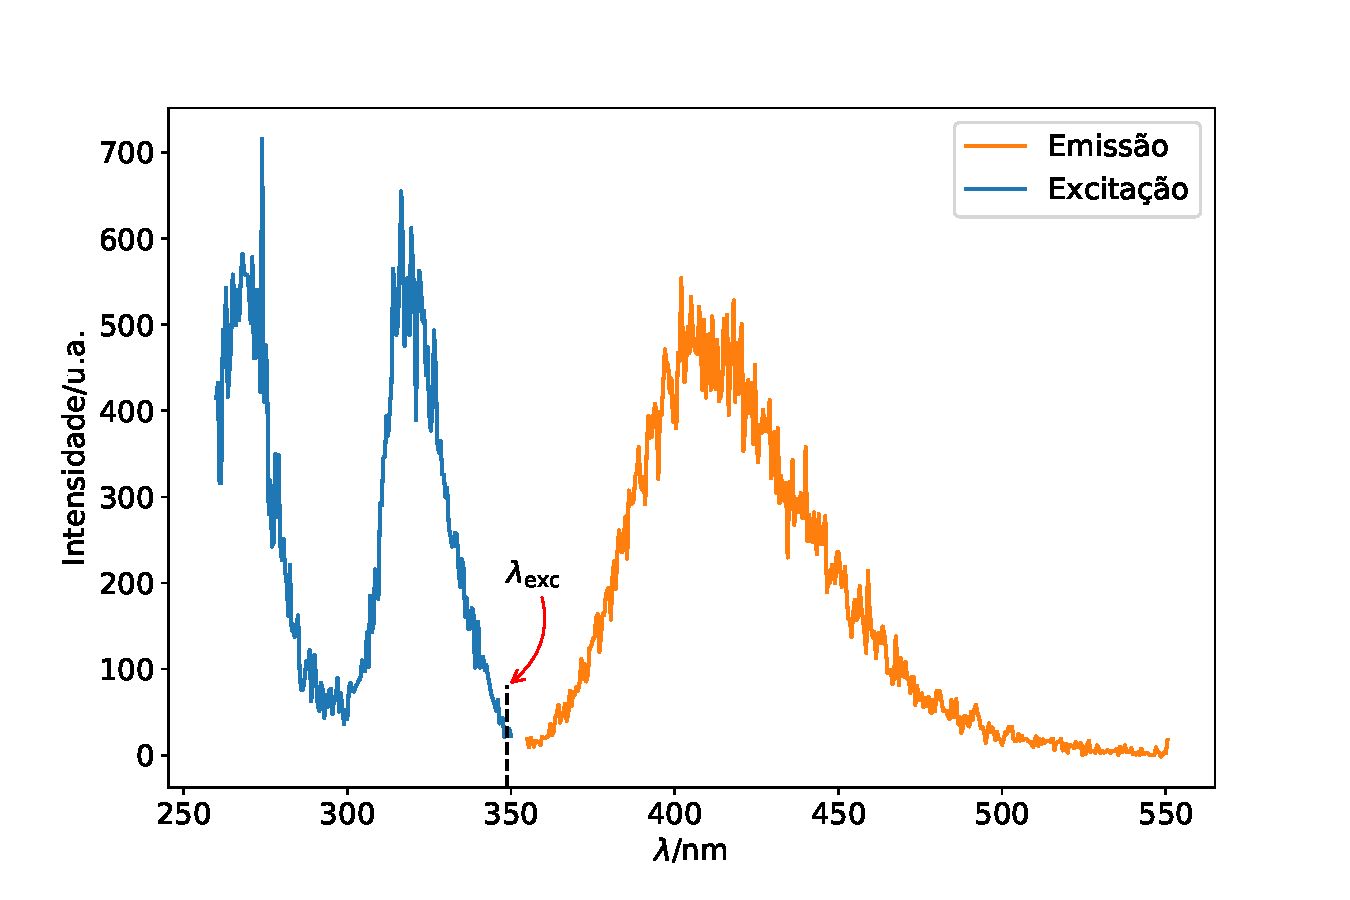
\includegraphics[width=0.7\textwidth]{imagens/fluor/emissao_excitacao}
		\caption{Curvas de emissão e excitação de NaSal. O comprimento de onda de excitação foi de 348 nm.}
		\label{fig:emissao_excitacao}
	\end{figure}

	Pode-se observar que há dois máximos de absorção, em 260 e 325 nm, e um máximo de emissão. Com o aumento da concentração de \TTAB{}, a intensidade do sinal de emissão também aumentou. Porém, como os sinais eram bastante ruidosos, ajustou-se uma função aos sinais, descrita na \autoref{eqn:ajuste_extremo}, para facilitar a visualização. As curvas ajustadas estão na \autoref{fig:emissao_nasal}.

	\begin{subequations}
		\begin{align}
		y &= y_0 + A e^{-e^{z} - z + 1} \\
		z &= \left( x - xc \right)/w 
		\end{align}
		\label{eqn:ajuste_extremo}
	\end{subequations}
	
	\begin{figure}[h]
		\centering
		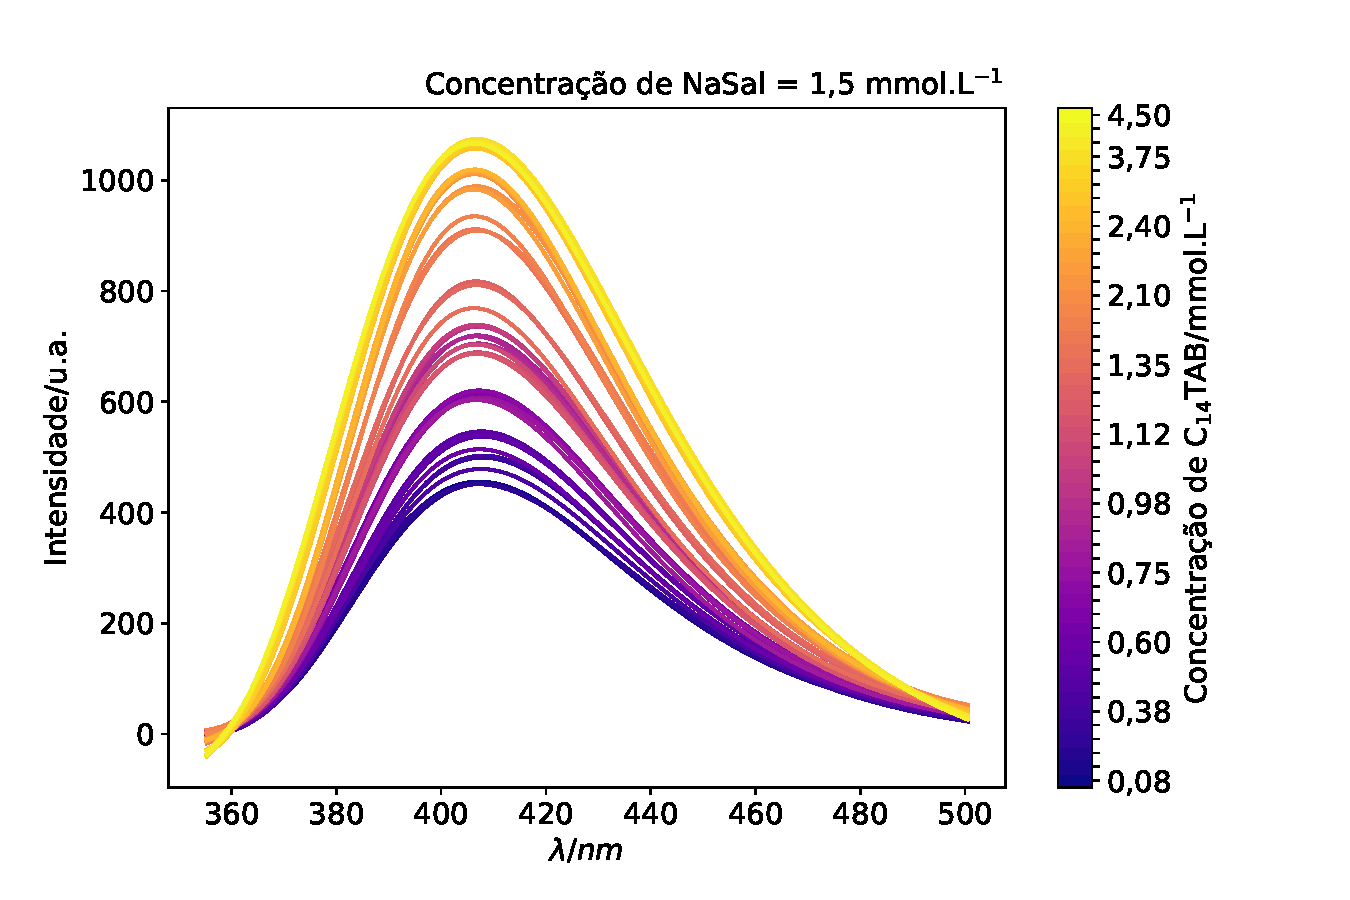
\includegraphics[width=0.7\textwidth]{imagens/fluor/emissao_nasal}
		\caption{Emissão de fluorescência de soluções de NaSal com \TTAB{} em concentrações crescentes.}
		\label{fig:emissao_nasal}
	\end{figure}
	
	Os máximos de todos os espectros de emissão foi em 411 nm, e por essa razão, esse comprimento de onda foi utilizado em todos os experimentos posteriores. O aumento de fluorescência da molécula de salicilato se deve à mudança do ambiente, quando se dirige à paliçada micelar. Isso aumenta o rendimento quântico do processo de fluorescência porque há uma menor proporção das moléculas excitadas que perde a sua energia por processos não radiativos, como colisão com moléculas de água.
	
	Portanto, a intensidade de fluorescência é dependente da inserção de salicilato nas micelas. Os processos de formação de micelas gigantes, observados por calorimetria, também ocorrem mediante a inserção de salicilato, logo os dois processos podem ser relacionados. A \autoref{fig:itc_fluorescencia} relaciona experimentos de ITC com a fluorescência em 411 nm.
	
	\begin{figure}[h]
		\centering
		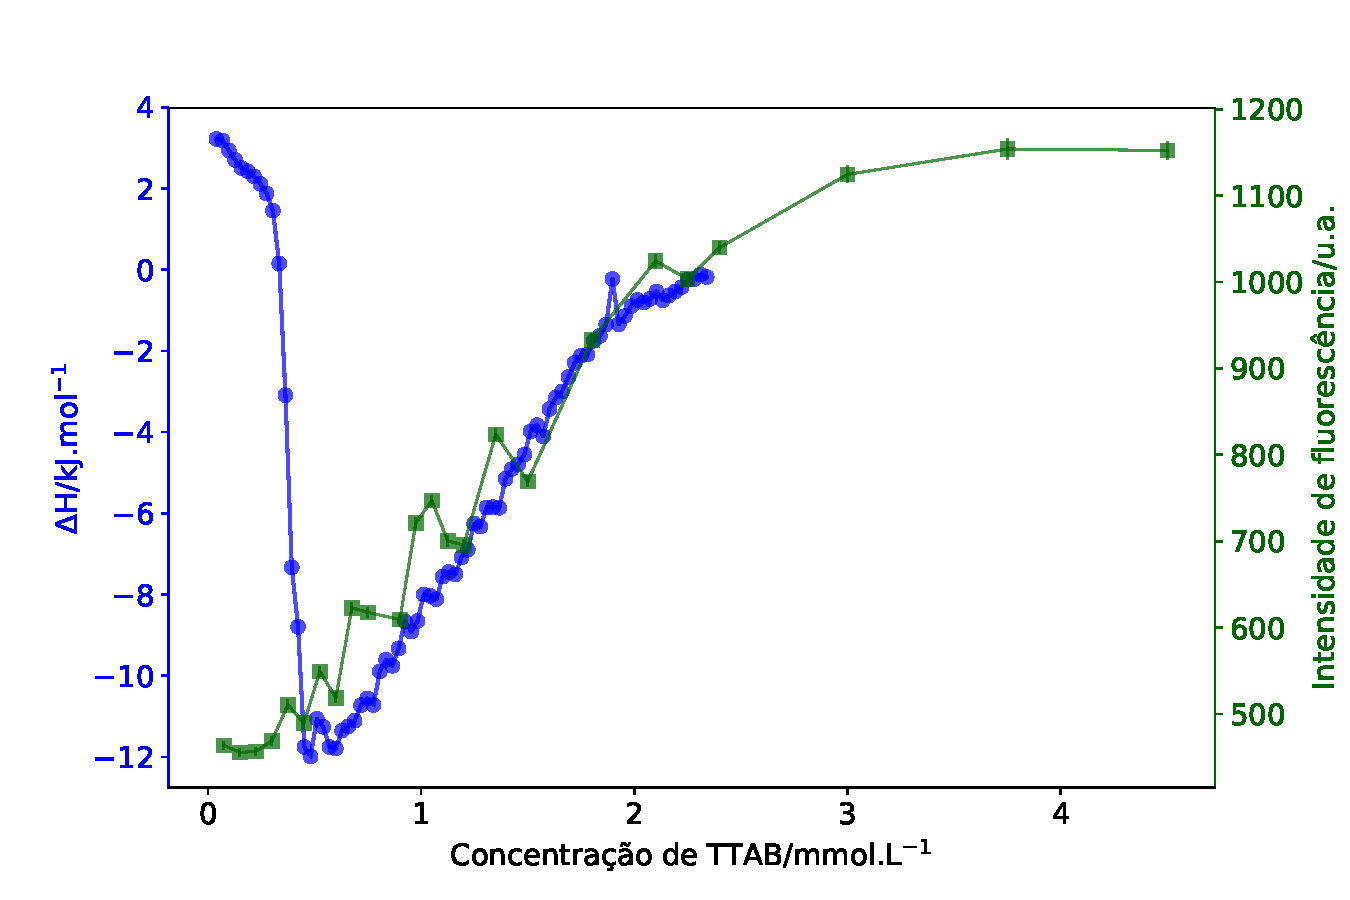
\includegraphics[width=0.7\textwidth]{imagens/fluor/itc_fluorescencia}
		\caption{Titulação de \TTAB 14 \mM{} em NaSal 1,5 \mM, comparado com o máximo de emissão, obtidos pela \autoref{fig:emissao_nasal}.}
		\label{fig:itc_fluorescencia}
	\end{figure}
	
	Na literatura, há um estudo que correlaciona o entalpograma com a viscosidade da solução, que se altera devido ao crescimento de micelas gigantes.\cite{Ito2015c} Esses valores de viscosidade foram extraídos para realizar mais comparações. A \autoref{fig:combinacao_propriedades} mostra as três propriedades em função da concentração de \TTAB.
	
	\begin{figure}[h]
		\centering
		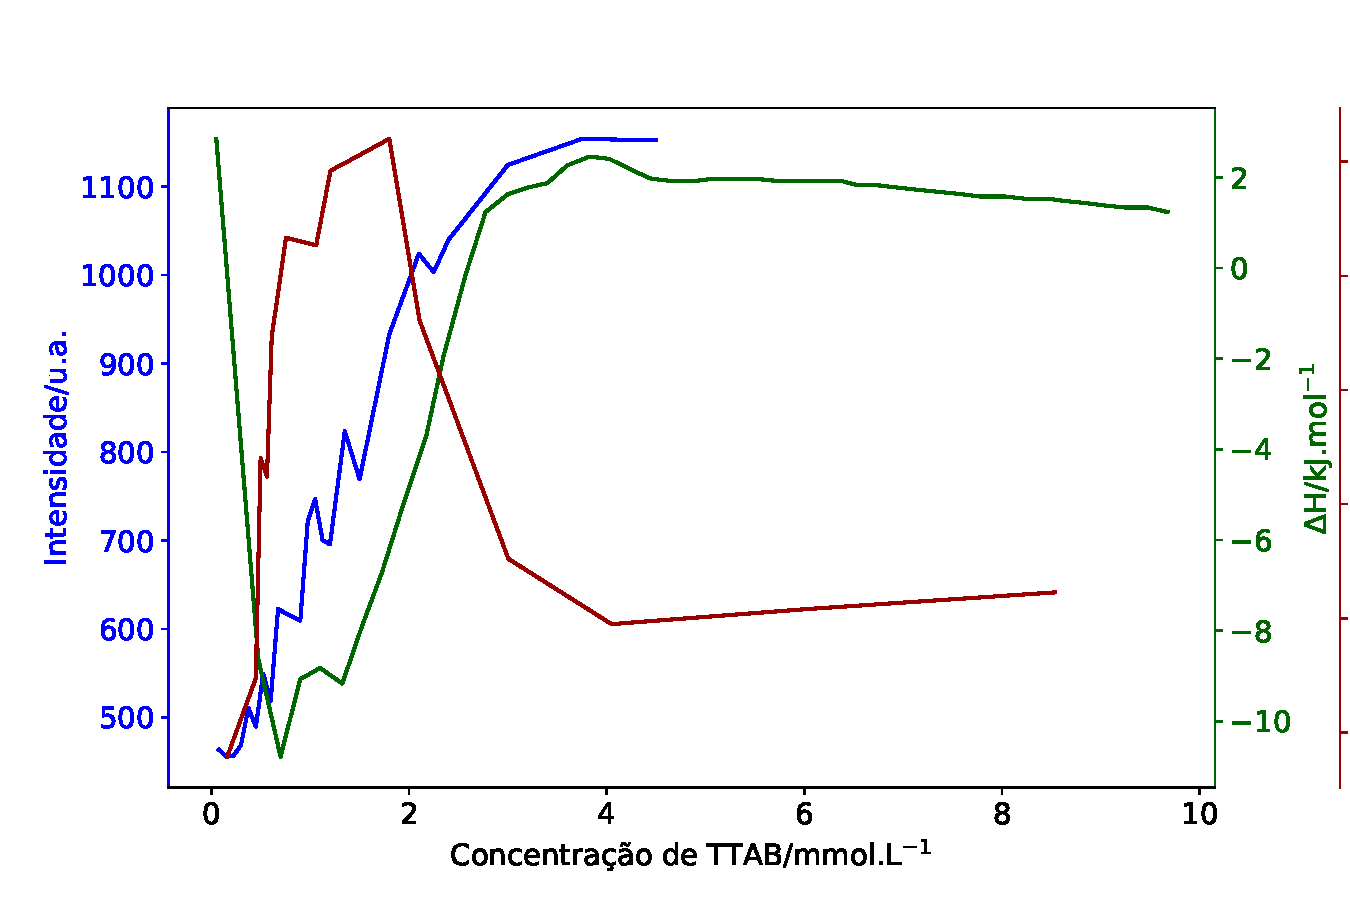
\includegraphics[width=0.7\textwidth]{imagens/fluor/combinacao_propriedades}
		\caption{Viscosidade, em mPa s, intensidade de fluorescência e entalpia de mistura de amostras com 1,5 \mM{} de NaSal e concentrações crescentes de \TTAB.}
		\label{fig:combinacao_propriedades}
	\end{figure} \index{resultados!fluorescência!correlação}
	
	Como todas as propriedades são dependentes da inserção de \Sal{} nas micelas, foi estudado se há uma correlação mais direta entre elas. A fluorescência é dependente da quantidade total de \Sal{} inserida. Já as entalpias de mistura individuais são dependentes da quantidade de \Sal{} incorporados às micelas em cada etapa. A viscosidade é uma propriedade dependente da concentração de NaSal, onde uma determinada concentração é capaz de fornecer uma ``quantidade'' de viscosidade específica, que a adição de mais \TTAB{} esgota. Assim, a integração do entalpograma seria proporcional à incorporação de \Sal{}, e a integração da viscosidade seria proporcional à quantidade total de viscosidade ``consumida'' por \TTAB. A  \autoref{fig:correlacoes_propriedades_zoom} mostra a correlação entre viscosidade e calorimetria integradas, e normalizadas pelo valor máximo, e a intensidade de fluorescência.
	
%	\begin{figure}
%		\begin{subfigure}{0.5\textwidth}
%			\centering
%			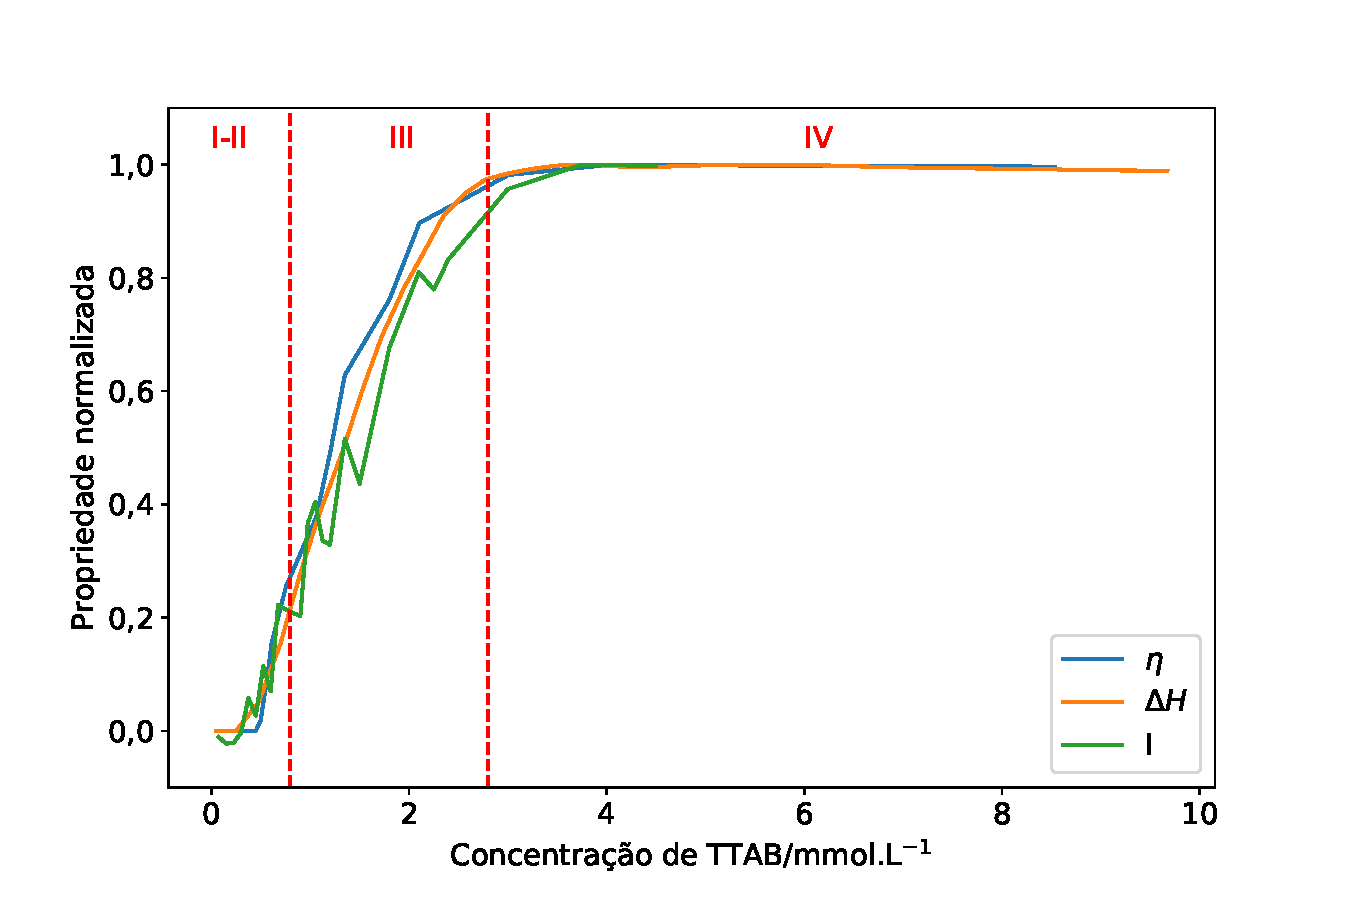
\includegraphics[width=0.7\textwidth]{imagens/fluor/correlacoes_propriedades}
%			\caption{}
%			\label{fig:correlacoes_propriedades_longe}
%		\end{subfigure}
	\begin{figure}[h]
		\centering
		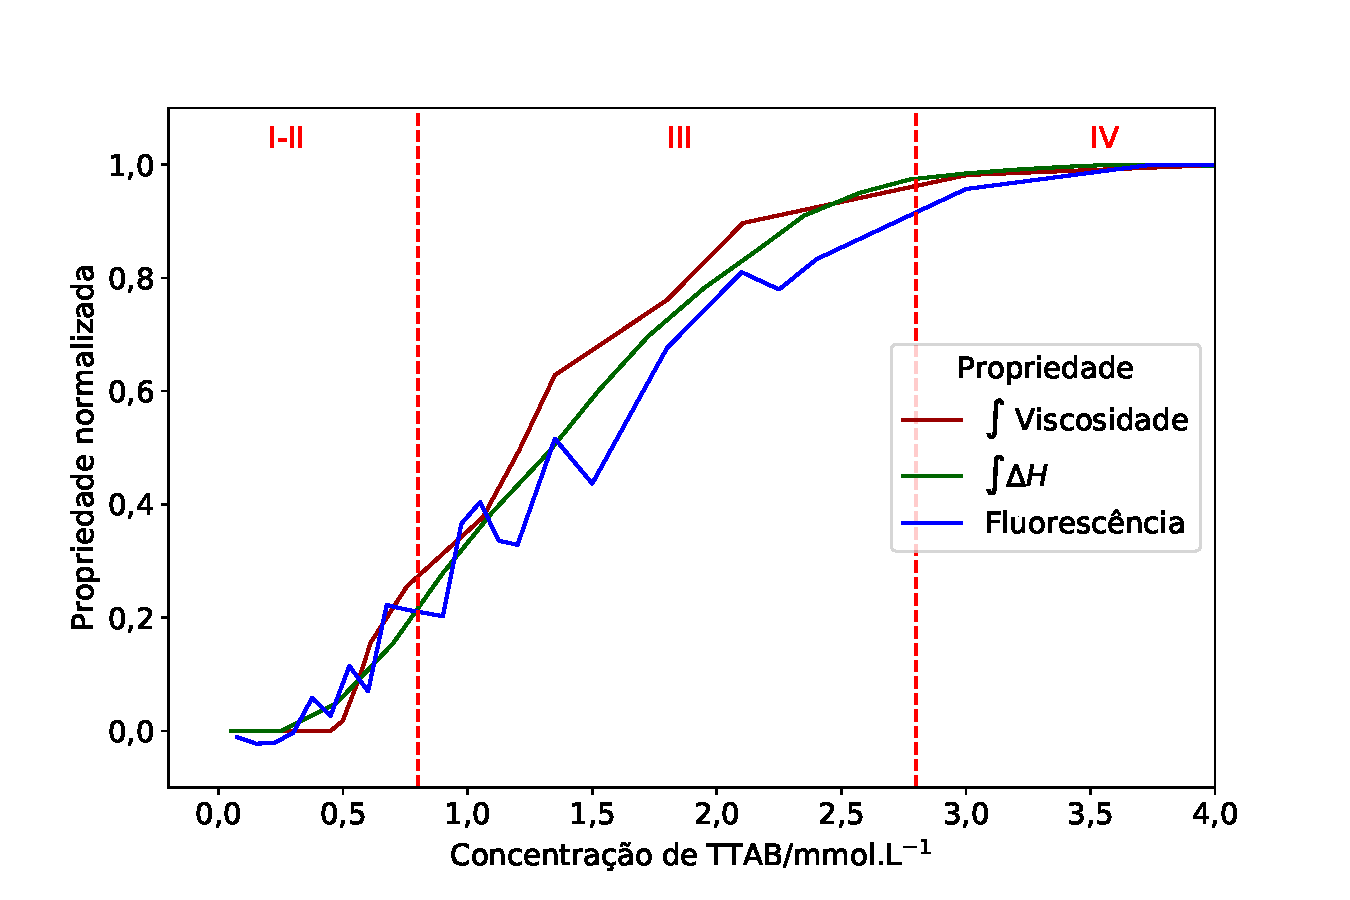
\includegraphics[width=0.7\textwidth]{imagens/fluor/correlacoes_propriedades_zoom}
		\caption{Correlações entre viscosidade integrada, entalpia integrada e intensidade de fluorescência, todas normalizadas}
		\label{fig:correlacoes_propriedades_zoom}
	\end{figure}
%	\caption{text}
%	\label{fig:correlacoes_propriedades}
%	\end{figure}
	
	É possível ver então que, de fato, as três propriedades estão correlacionadas, e é possível relacionar uma determinada intensidade de fluorescência com a quantidade de salicilato incorporado, a viscosidade e a calorimetria.

	\FloatBarrier	
	
	\section{Cinética medida por fluorescência} \index{resultados!fluorescência!cinética}
	
	Foram realizados estudos de cinética misturando-se duas soluções, de forma que sua mistura resulte numa solução com micelas gigantes. Uma maneira de se fazer isso é misturando uma solução de NaSal 1,5 \mM{} e outra contendo tanto NaSal 1,5 \mM{} quanto \TTAB{} 1,7 \mM. Essa concentração de \TTAB{} está longe da região do mínimo, com baixa viscosidade. Quando misturadas, a concentração de \TTAB{} será diminuída pela metade, atingindo a concentração de 0,85 \mM{}, próximo ao mínimo. Logo, observaria-se o crescimento das micelas, através de um salto de concentração, em paralelo a experimentos de saltos de temperatura ou pressão.\cite{Hoffmann2012a} A \autoref{fig:itc_experimento_cinetica} ilustra a mistura que irá ocorrer, e sua relação com o entalpograma e a fluorescência.
	
	\begin{figure}[h]
		\centering
		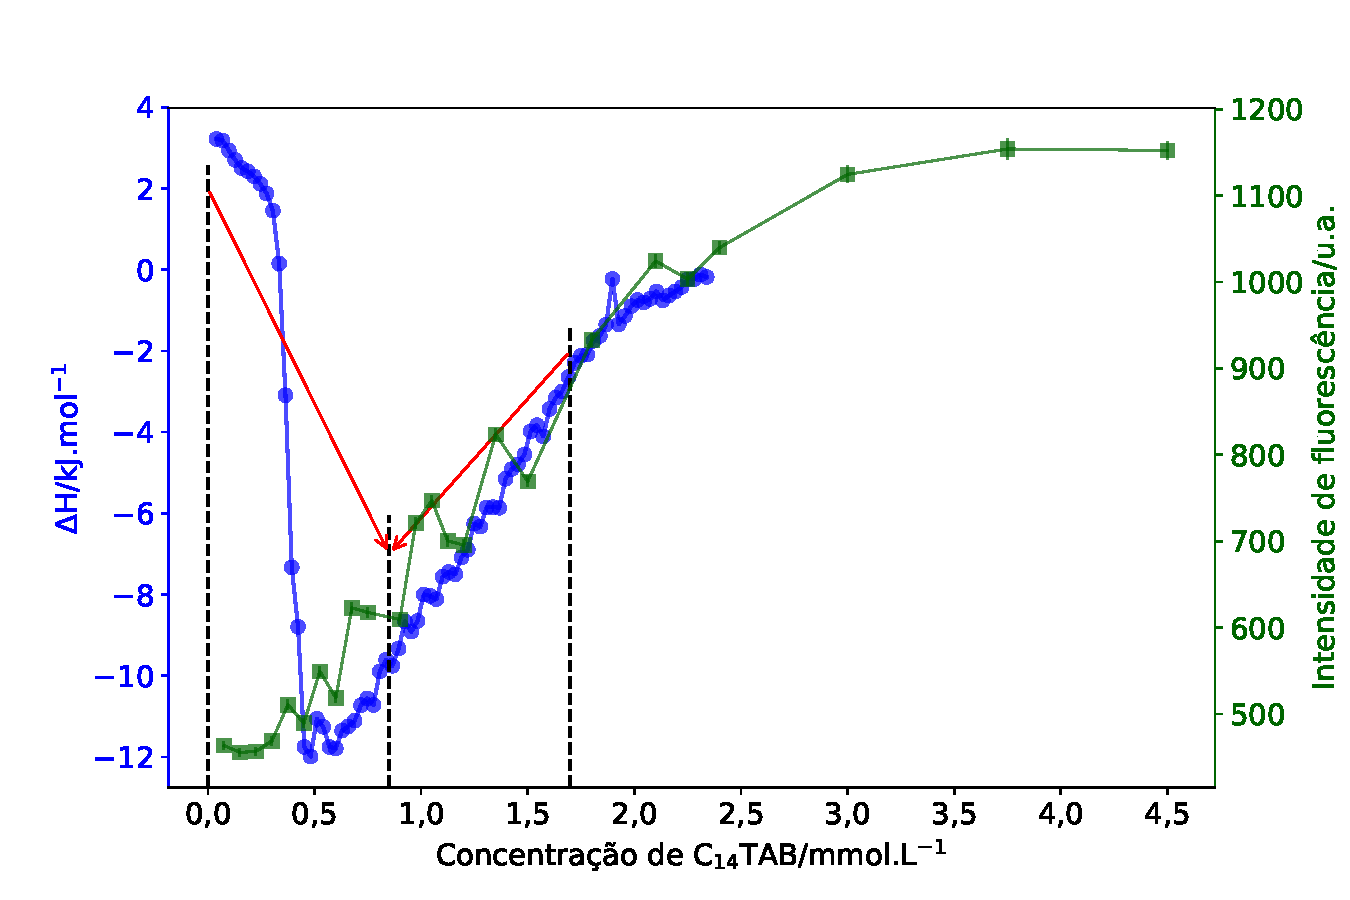
\includegraphics[width=0.7\textwidth]{imagens/fluor/itc_experimento_cinetica}
		\caption{Entalpograma e fluorescência de NaSal. As setas começam da composição que estará presente em cada seringa, antes da injeção no \emph{stopped-flow}, e indicam qual é o estado final após a injeção. A concentração de NaSal é de 1,5 \mM{} em ambas as soluções.}
		\label{fig:itc_experimento_cinetica}
	\end{figure}
	
	Com as amostras prontas, montou-se o aparato descrito na seção experimental (\autoref{sec:experimental_fluor_resolvida}), e foram injetadas as soluções. Em parte dos experimentos, a cela de medida foi lavada com água até que todo sinal de fluorescência do salicilato desaparecesse. Na outra parte, a cela não foi limpa, de modo a observar se havia diferença no sinal de fluorescência imediatamente após a injeção, e após alguns minutos.
	
	Como resultado de cada análise, um mapa de cor é obtido, contendo os espectros medidos em y, o tempo em x, e as cores correspondendo à intensidade do sinal. Um mapa de cor padrão se encontra na \autoref{fig:mapa_cor_fluorescencia}.
	
	\begin{figure}[h]
		\centering
		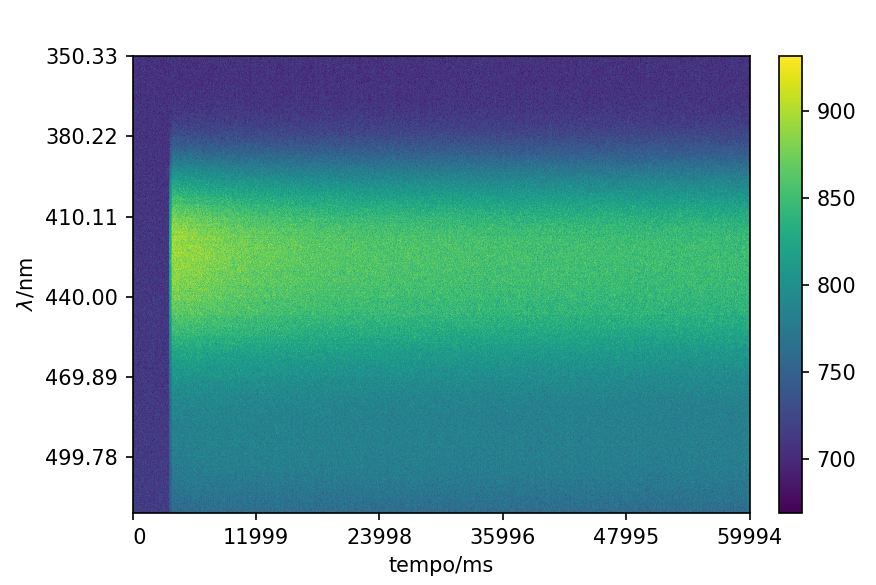
\includegraphics[width=0.6\textwidth]{imagens/fluor/mapa_cor_am49}
		\caption{Mapa de cor obtido após um experimento de cinética, mostrando a intensidade de fluorescência em função do tempo e do comprimento de onda. É possível observar a banda de fluorescência, com máximo em 411 nm, vista na \autoref{fig:emissao_excitacao}, e como a intensidade diminui gradativamente com o tempo}
		\label{fig:mapa_cor_fluorescencia}
	\end{figure}
	
	Desse mapa, foi retirada a variação da intensidade em 411 nm, o máximo do sinal, em função do tempo. Cada sinal é extremamente ruidoso, devido ao baixo tempo de integração de 6 ms.
	A \autoref{fig:curva_inicio_final_cortada} mostra essa seção do mapa de cor, evidenciando o ponto de injeção, onde a intensidade de fluorescência aumenta.
	
	\begin{figure}[h]
		\centering
		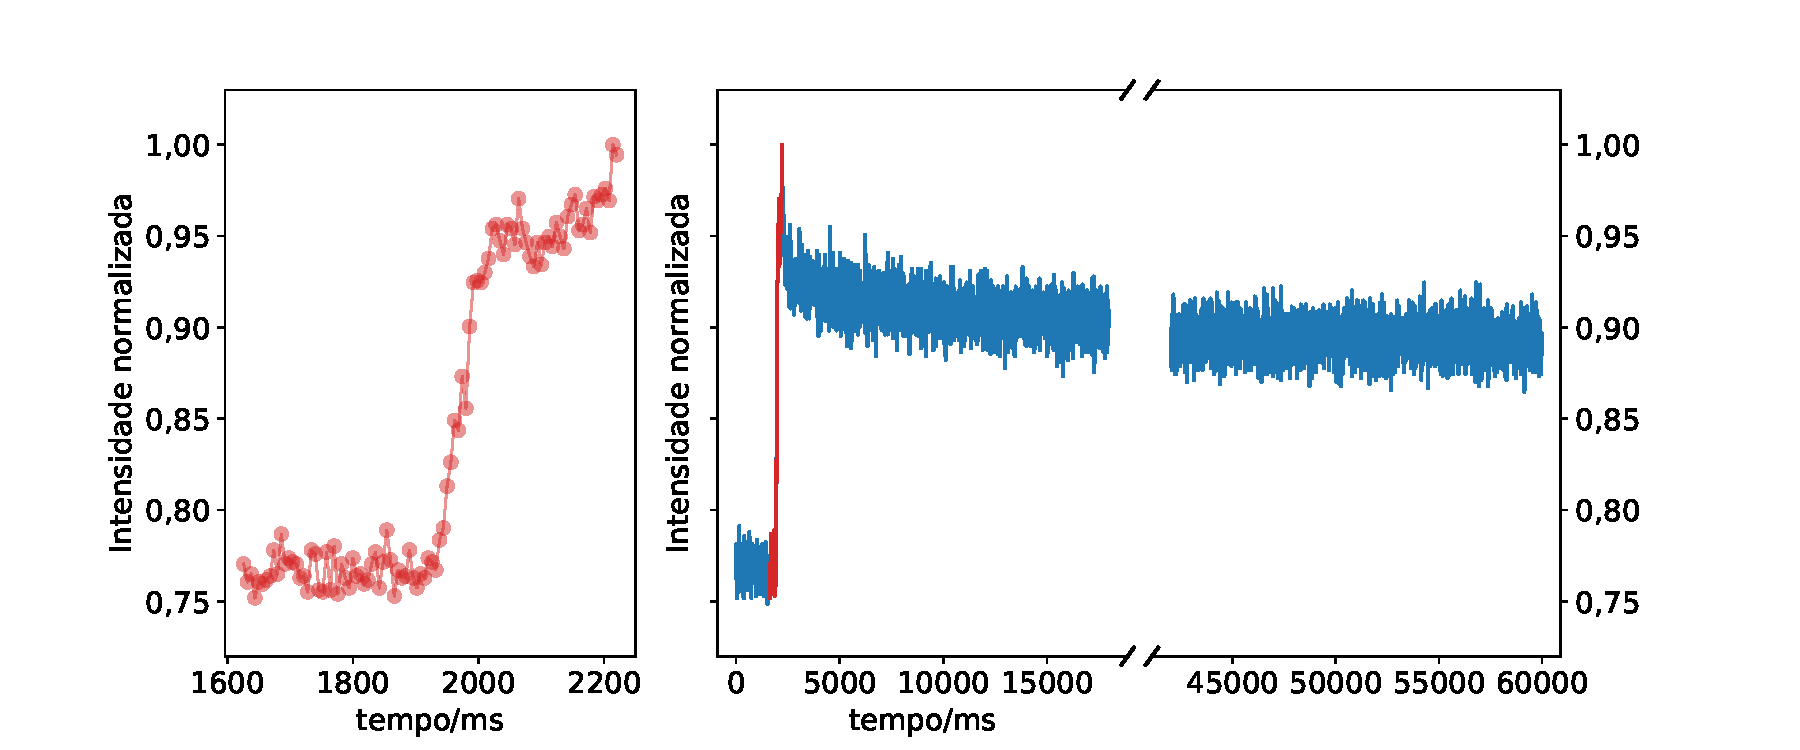
\includegraphics[width=\textwidth]{imagens/fluor/curva_inicio_final_cortada}
		\caption{Seção em 411 nm do mapa de cor da  \autoref{fig:mapa_cor_fluorescencia}. Em vermelho, à esquerda, está a região onde ocorre a injeção. À direita, o perfil de fluorescência contem a região pré-injeção, a região de injeção, em vermelho, e a região de pós-injeção, que decai gradativamente em função do tempo.}
		\label{fig:curva_inicio_final_cortada} 
	\end{figure}
	
	Cada curva possui três regiões distintas. A primeira, antes da injeção, corresponde ao sinal de fluorescência do porta-amostra. Quando é feita a injeção, a intensidade de fluorescência aumenta abruptamente, devido à introdução de \TTAB{} ao porta-amostra. A terceira região começa após o pico de intensidade, onde há, aparentemente, um decaimento gradual e bastante lento de fluorescência.
	
	A região de inflexão foi analisada para obter-se o tempo de mistura das soluções. Possivelmente esse tempo de mistura esteja relacionado ao crescimento micelar, pois ambos ocorrem em escalas de tempo próximas às observadas por SAXS. Além disso, a região após o máximo, onde ocorre o decaimento, também foi analisada, de modo a determinar se esse decaimento se deve à lenta transição das micelas de uma seringa para o estado final, próximo ao máximo de viscosidade. 
	
	Cada curva foi alisada pelo método de Savitzky-Golay de segundo grau, utilizando uma janela variável para cada região da curva. Para a região de inflexão, foi utilizada uma janela pequena, com aproximadamente a metade do número de pontos da região de inflexão. Para a região de decaimento, foi utilizada uma janela de 201 pontos, muito maior, para aumentar a intensidade de alisamento. A \autoref{fig:decaimento_fluorescencia_mg1} mostra como a utilização de Savtizky-Golay é essencial para a análise das curvas. 

	\begin{figure}[h]
		\begin{subfigure}{\textwidth}
			\centering
			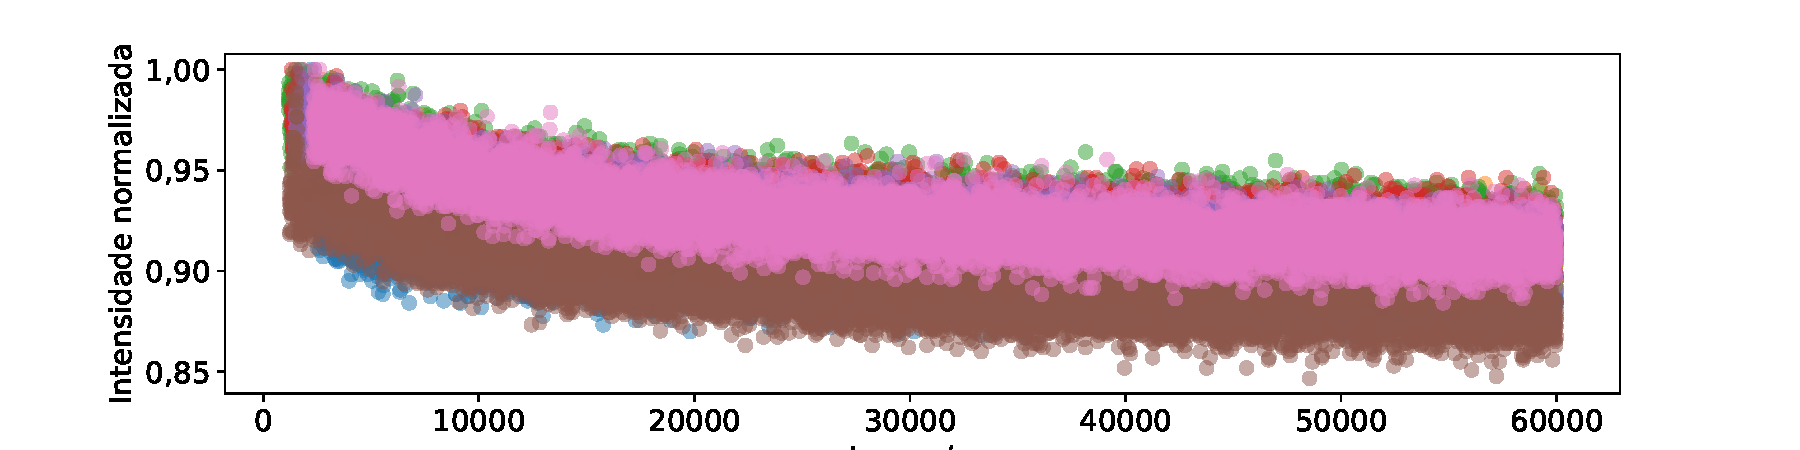
\includegraphics[width=\textwidth]{imagens/fluor/decaimento_mg1}
			\caption{Sem Savitzky-Golay}
			\label{fig:decaimento_mg1}
		\end{subfigure}

		\begin{subfigure}{\textwidth}
			\centering
			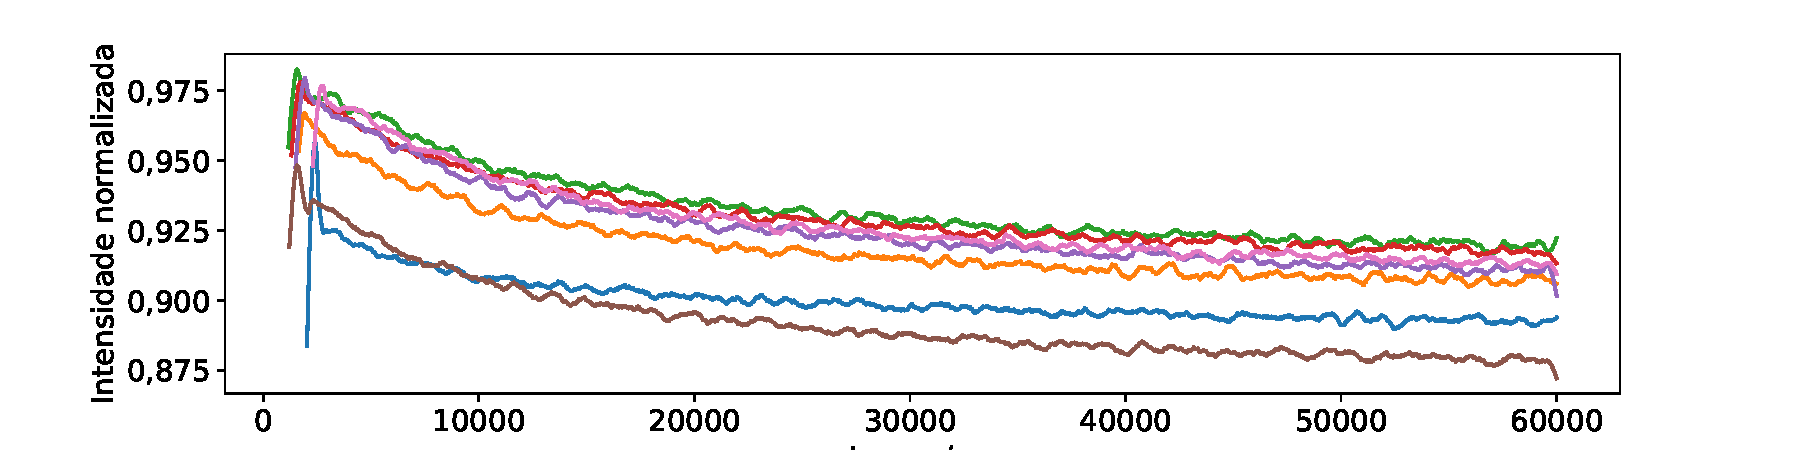
\includegraphics[width=\textwidth]{imagens/fluor/decaimento_mg1_SG}
			\caption{Com Savitzky-Golay}
			\label{fig:decaimento_mg1_sg}
		\end{subfigure}
		
		\caption{Intensidades de fluorescência após a injeção de \TTAB{} 1,7 \mM{} com NaSal 1,5 \mM{} em NaSal 1,5 \mM{}, sem alisamento (\autoref{fig:decaimento_mg1}) e com alisamento (\autoref{fig:decaimento_mg1_sg}) de segundo grau e janela de 201 pontos.}
		\label{fig:decaimento_fluorescencia_mg1}
	\end{figure}	


	\FloatBarrier
	
	Como comparativo, foram analisadas injeções de NaSal 3,0 \mM{} em água, e com soluções 4\% e 10\% de sacarose (em ambas as seringas), para simular a viscosidade das micelas. Assim, observaria-se se há decaimento de fluorescência, e se há diferenças na região de inflexão. Essas análises serão denominadas, de forma geral, como o branco do experimento.  Além disso, foram analisadas as misturas de \TTAB{} 1,7 \mM{} e NaSal 1,5 \mM{} em água, ao invés de NaSal, para observar se a intensidade de fluorescência basal interfere nos parâmetros medidos.
	
	A \autoref{fig:fluorescencia_comparativo_cineticas} mostra cinco curvas de decaimento descritivas das cinco diferentes combinações utilizadas na mistura.
	
	\begin{figure}[h]
		\centering
		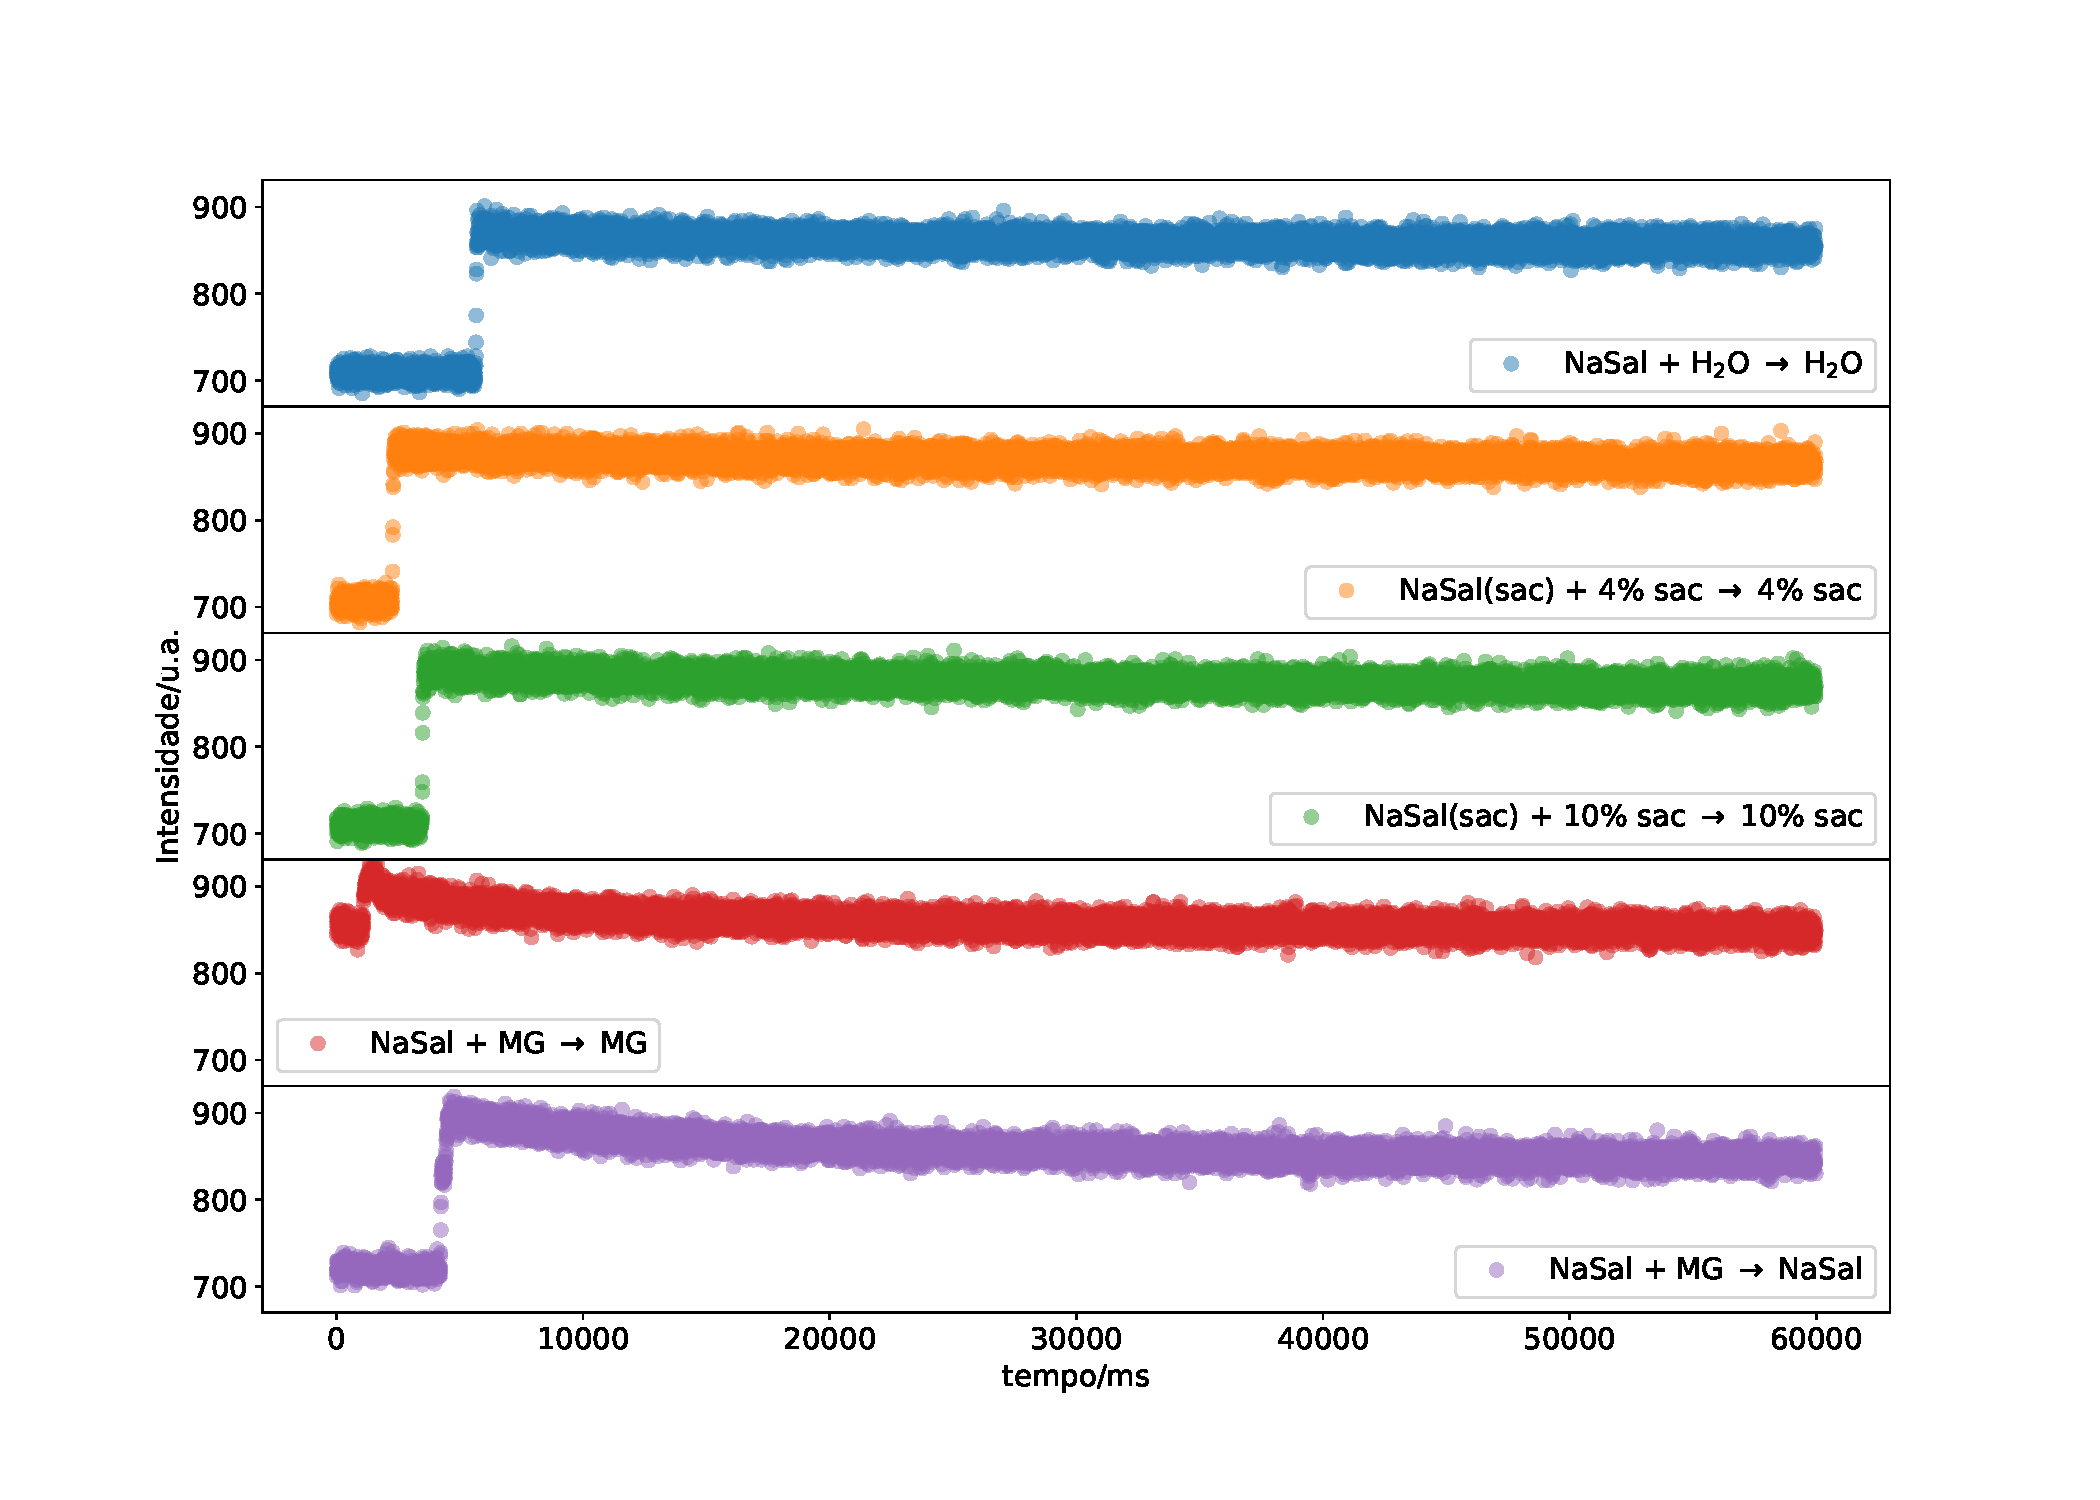
\includegraphics[width=\textwidth]{imagens/fluor/fluorescencia_comparativo}
		\caption{Perfis de fluorescência em 411 nm para cinco diferentes experimentos realizados de forma a testar se há diferença entre os perfis de mistura na presença de \TTAB.}
		\label{fig:fluorescencia_comparativo_cineticas}
	\end{figure}
	
	Os tempos de aumento de fluorescência foram medidos manualmente, contando-se o número de pontos da linha base até o máximo de fluorescência. Já a região de decaimento após o alisamento foi analisada pelo ajuste de várias equações de decaimento, até observar-se, pelo valor de \(R^2\) e os erros dos parâmetros, que o melhor modelo é o de decaimento exponencial simples (\autoref{eqn:decaimento_exponencial}). A \autoref{tab:params_ajuste_decaimento} mostra o valor médio do coeficiente de determinação para os ajustes exponenciais, o valor médio da constante de decaimento e o valor médio do tempo de injeção.
	
	\begin{table}[h]
		\IBGEtab{%
			\caption{Parâmetros médios dos ajustes exponenciais, e da contagem da região de inflexão, para várias diferentes misturas. MG significa solução de \TTAB{} 1,7 \mM{} e NaSal 1,5 \mM. As misturas com MG ocorreram com NaSal 1,5 \mM, e com os solventes, iguais em ambas as seringas, ocorreram com NaSal 3,0 \mM.}
			\label{tab:params_ajuste_decaimento}
		}%
		{%
			\begin{tabular}{p{4cm} c c c c}
				\toprule
				Mistura                                        & replicatas & \(R^2\) & \(t_1\)/ms        & \(t_{\mathrm{inj}}\)/ms \\ \midrule
				NaSal + \agua{} \(\to\) \agua                  & 8          & 0.934   & 23100 \(\pm\) 234 & 60 \(\pm\) 24           \\
				NaSal\textsubscript{sac} \(\to\) Sacarose 4\%  & 7          & 0.946   & 25600 \(\pm\) 240 & 64 \(\pm\) 9            \\
				NaSal\textsubscript{sac} \(\to\) Sacarose 10\% & 5          & 0.956   & 26100 \(\pm\) 228 & 44 \(\pm\) 14           \\ \midrule
				MG + NaSal \(\to\) NaSal                       & 10         & 0.987   & 14540 \(\pm\) 48  & 64 \(\pm\) 9            \\
				MG + NaSal \(\to\) \agua                       & 6          & 0.987   & 14190 \(\pm\) 41  & 62 \(\pm\) 34           \\ \bottomrule
			\end{tabular}
		}{}
	\end{table} \index{resultados!fluorescência!ajuste}
	
	Observa-se que há uma diferença significativa tanto no coeficiente de determinação quanto na constante de decaimento entre as injeções com e sem \TTAB{}. Os valores menores de \(R^2\) e os erros maiores se devem à menor taxa de decaimento, isso é, a curva é mais próxima a uma reta horizontal.  Porém, não se observa uma diferença entre os tempos de injeção. Isso indica que o crescimento micelar ocorre após a injeção, e prossegue bastante lentamente.
	
	A hipótese de que o fenômeno que concede o decaimento exponencial é o crescimento micelar foi testado de uma maneira bastante simples. Um papel foi colocado na frente da fonte de luz. Caso o decaimento seja devido ao crescimento micelar, o mesmo deve prosseguir sem a incidência de radiação. Caso contrário, é possível que a incidência de luz esteja resultando em alguma modificação no sistema. A \autoref{fig:fluorescencia_buraco} mostra a curva resultante, e a junção das duas regiões pré- e pós-bloqueio.
	
	\begin{figure}[h]
		\centering
		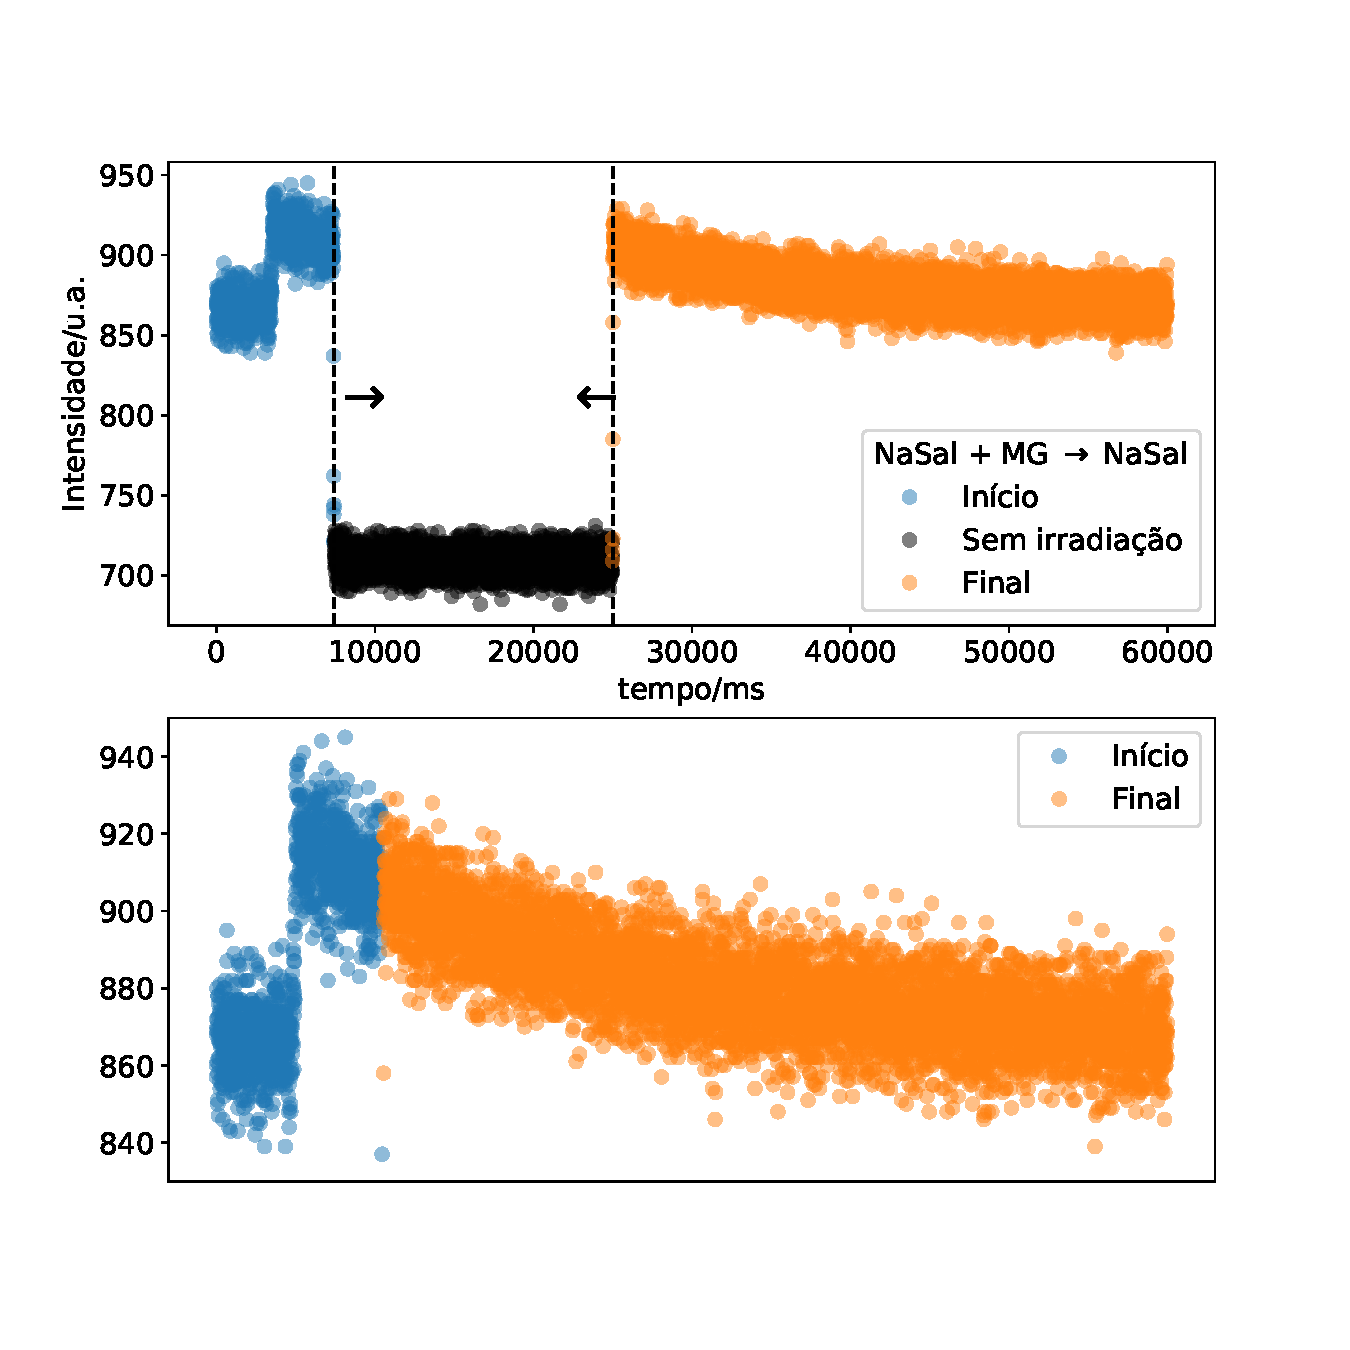
\includegraphics[width=0.7\textwidth]{imagens/fluor/buraco}
		\caption{Intensidade de fluorescência em função do tempo. Durante o experimento, foi colocada uma folha de papel entre a fonte de luz e o porta-amostra, que foi retirada pouco tempo depois. As duas seções da curva foram juntadas, mostrando que o decaimento não ocorre sem a irradiação.}
		\label{fig:fluorescencia_buraco}
	\end{figure}
	
	Observa-se claramente que o decaimento recomeça assim que a luz começa a reincidir na amostra. Isso coloca em dúvida as conclusões observadas anteriormente. Possivelmente, o decaimento se deve a algum fenômeno fotoquímico ou fotofísico desconhecido.
	
	Como o decaimento aparenta ocorrer em tempos muito longos, foi utilizado outro equipamento para comparar os resultados, utilizando tempos de integração de 1s, mas com uma incidência de radiação muito menos intensa. A \autoref{fig:fluor_claudia} mostra as curvas observadas para todas as misturas utilizadas na  \autoref{tab:params_ajuste_decaimento}.
	
	\begin{figure}[h]
		\centering
		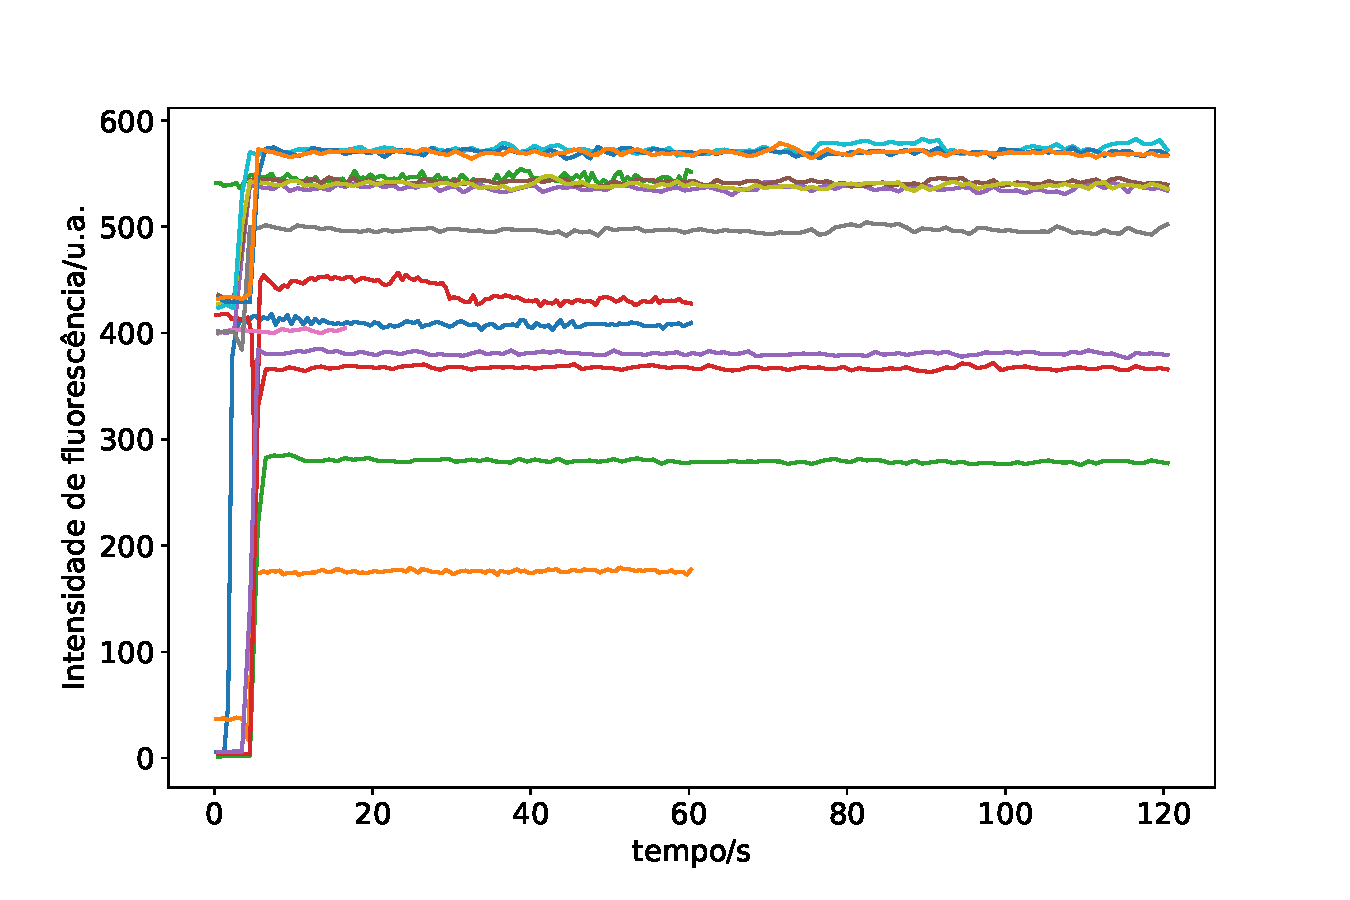
\includegraphics[width=0.7\textwidth]{imagens/fluor/exp_claudia}
		\caption{Evolução da fluorescência em função do tempo em outro equipamento, com tempos de integração de 1s, para as diferentes injeções indicadas na  \autoref{tab:params_ajuste_decaimento}. Não há diferença no decaimento das curvas.}
		\label{fig:fluor_claudia}
	\end{figure}
	
	Claramente não é observado nenhum decaimento. Essa informação, contraditória com os experimentos anteriores, indica que não foi observado, em nenhuma instância até agora, o crescimento micelar, somente processos relacionados ao processo de análise. Ou o crescimento micelar ocorreu em muito pouco tempo, como nos experimentos de SAXS, ou a incidência de luz auxilia nesse processo, ou o crescimento micelar não pode ser observado por fluorescência.
	
	\section{Conclusão parcial}	 \index{conclusões!fluorescência}
	
	Observou-se que a fluorescência de \Sal{} aumentava com o aumento da concentração de \TTAB. Isso foi atribuído à uma menor quantidade de \Sal{} em solução, e o ponto onde a fluorescência começa a subir é o mesmo ponto onde começa o crescimento micelar. Foi possível correlacionar isso a outras propriedades, a viscosidade e os resultados calorimétricos.
	
	Porém, resultados contraditórios mostram que a determinação de cinética de crescimento micelar através da fluorescência e stopped-flow, é experimentalmente difícil, e estudos posteriores, com técnicas experimentais mais refinadas, serão necessários para determinar, com total certeza, se o crescimento micelar pode ser diretamente observado por fluorescência.
	
	\chapter{Conclusões sobre a cinética de crescimento} \index{conclusões!cinética}
	
	Estudos de cinética de crescimento foram realizados tanto por SAXS resolvido no tempo quanto por fluorescência junto de um aparato de stopped-flow.
	
	Nos experimentos com SAXS, não foi possível observar o processo completo de crescimento micelar. Ou o processo termina por volta de 60 ms após a mistura, ou a concentração é tão alta que a técnica de SAXS, na faixa de \q{} utilizada, não é capaz de diferenciar faixas de tamanho maiores. Para essas análises, utilizou-se o ajuste de um modelo altamente complexo, descrito detalhadamente nos \autoref{sec:modelo_MG_matematica} e \autoref{sec:modelo_MG_python}. Esse modelo poderá ser utilizado posteriormente pelo grupo, e por outros, para a análise de objetos alongados \emph{core-shell} como micelas gigantes.
	
	Nos experimentos de fluorescência, observou-se alterações no decaimento de intensidade de fluorescência entre experimentos onde ocorre o crescimento micelar, e quando ocorre somente a diluição de NaSal. Porém, esses resultados foram invalidados por experimentos posteriores, que influenciaram a incidência de radiação no porta-amostra, levantando a hipótese de que a fonte utilizada está interferindo nos processos medidos. Para determinar isso, será necessário realizar experimentos mais refinados, com controle eletrônico de injeção com alta resolução temporal, controle de parada de amostra no porta-amostra (\emph{dead-stop}), sistemas de aquisição menos ruidosos e um método de excitação mais seletivo ao comprimento de onda desejado.
	
\FloatBarrier